\documentclass{amsart}
\usepackage{master}
\begin{document}
\title{Seiberg-Witten theory on four-manifolds}
\author{Lectures by Francesco Lin\\
Notes by Jackson Van Dyke}
\thanks{All errors introduced are my own}
\maketitle

\section{The intersection form and motivation}

Throughout, $X$ will be a closed oriented smooth four-manifold. 
The intersection form is a bilinear pairing 
\begin{equation}
Q_X:H^2\left( X , \ZZ \right)/\Tors 
\tp H^2\left( X , \ZZ \right)/\Tors = \ZZ^{b_2\left( X \right)} \fromto\ZZ
\end{equation}
which maps $\left( \al , \b \right) \mapsto \left( \al \cupp \b \right)\left[ X \right]$
since $\left( \al \cupp \b \right) \in H^4$ whereas 
$\left[ X \right]\in H_4$.
We can also think about this in the following slightly different way:

\begin{thm}
Suppose $\al , \al'\in H^2$, and suppose we have some surface $\Sigma$ representing the Poincar\'e
dual of $\al$, $\PD\left[ \al \right] \in H_2$ and some surface $\Sigma'$ representing
the Poincar\'e dual of $\al'$, $\PD\left[ \al' \right] \in H_2$.
Then 
\begin{equation}
Q\left( \al , \al' \right) = \#\left( \Sigma \cap \Sigma' \right)
\end{equation}
\end{thm}

\begin{exm}
We consider some preliminary examples:
\begin{enumerate}
\item Consider $S^4$, then we have $H^2 = 0$, so $Q_X = 0$
\item Consider $S^2 \times S^2$ then $H^2 = \ZZ \dsum \ZZ$, so
\begin{equation}
Q_X = 
\begin{pmatrix}
0 & 1 \\ 1 & 0
\end{pmatrix}
\end{equation}
\item Consider $\CP^2$, then we have $H^2 = \ZZ = \left[ \CP^2 \right]$, so
$Q_X = \left[ 1 \right]$. 
\item Now reverse the orientation to get $\barr{\CP^2}$. We still have
$H^2 = \ZZ$, but now $Q_X = \left[ -1 \right]$.
\end{enumerate}
\end{exm}

We now consider some preliminary properties of the intersection form

\begin{thm}
\begin{enumerate}
\item $Q_X$ is unimodular, that is, it has determinant $\pm 1$.\footnote{
This can be shown using Poincar\'e duality.}
\item Take $X$, $X'$ then we remove a copy of $D^4$ from both, and glue them together to get
$X\# X$. This is called the \emph{connected sum}.
We have the following:
\begin{equation}
Q_{X\# X'} = Q_X \dsum Q_{X'}
\end{equation}
\end{enumerate}
\end{thm}

\begin{exm}
If $X = \CP^2 \# \barr{\CP^2}$, then we get the following intersection form:
\begin{equation}
Q_X = 
\begin{pmatrix}
1 & 0 \\ 0 &-1
\end{pmatrix}
\end{equation}
\end{exm}

\begin{rmk}
The operation of taking $\cdot \# \barr{\CP^2}$ is what an algebraic geometer would call blowing up
as in \cref{fig:blowing_up}.
\begin{figure}
\centering
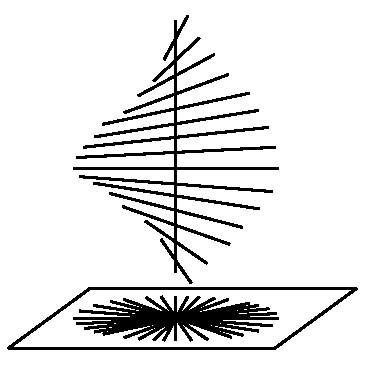
\includegraphics[width=0.5\textwidth]{blowup.png}
\caption{The blowing up procedure.}
\label{fig:blowing_up}
\end{figure}
\end{rmk}

\begin{thm}[Freedman]
Let $X$, $X'$ be smooth, and simply-connected.
Then $X$ is homeomorphic to $X'$ iff $Q_X \simeqq Q_{X'}$.
\end{thm}

The proof of this theorem is very challenging. 

\subsection{Invariants coming from the intersection form}

Consider the following three invariants:
the rank of $Q_X$, which is $b_2\left( X \right)$, 
the signature of $Q_X\tp \RR$, which is the number of positive eigenvalues 
minus the number of negative eigenvalues, 
and the parity. This is even if $Q_X\left( \al , \al  \right)\in 2\ZZ$ for all $\al$, 
and otherwise $Q_X$ is odd.

\begin{exm}
So far we haven't seen very many exciting intersection forms. 
As an example, we offer the following:
\begin{equation}
E_8 = 
\begin{pmatrix}
2 & 1 & 0 & 0 & 0 & 0 & 0 & 0 \\
1 & 2 & 1 & 0 & 0 & 0 & 0 & 0 \\
0 & 1 & 2 & 1 & 0 & 0 & 0 & 0 \\
0 & 0 & 1 & 2 & 1 & 0 & 0 & 0 \\
0 & 0 & 0 & 1 & 2 & 1 & 0 & 1 \\
0 & 0 & 0 & 0 & 1 & 2 & 1 & 0 \\
0 & 0 & 0 & 0 & 0 & 1 & 2 & 0 \\
0 & 0 & 0 & 0 & 1 & 0 & 0 & 2
\end{pmatrix}
\end{equation}
This is positive definite, even, and unimodular, with $\sigma\left( Q \right) = 8$.
\end{exm}

\begin{rmk}
We don't typically see such positive definite things in low-dimensional topology.
\end{rmk}

\begin{thm}[Donaldson]
If $X$ is smooth and the intersection form is positive definite, then the intersection
form is diagonal. 
\end{thm}

We will prove this later.

\begin{cor}[Donaldson-Freedman-Serre]
Suppose $X$, $X'$ are smooth and simply connected. 
Then $X$ and $X'$ are homeomorphic iff they have the same rank, 
signature, and parity.
\end{cor}

Our generic goal here is to construct infinitely many smooth 
$4$-manifolds which are homeomorphic but not diffeomorphic.
To show these are homeomorphic we will use the above theorem, 
and to show they are not diffeomorphic we will use Seiberg-Witten (SW) theory.

\begin{exm}
Consider the $K3$ surface:
\begin{equation}
\left\{ x_0^4 + x_1^4 + x_2^4 + x_3^4 = 0 \right\} \sub \CP^3
\end{equation}
This is simply connected, that is $\pi_1 = 0$, 
and has the following intersection form:
\begin{equation}
Q_{K3} = -2 E_8 \dsum 3 
\begin{pmatrix}
0 & 1 \\ 1 & 0
\end{pmatrix}
\end{equation}
This is even, has rank $22$, and signature $-16$.
This can be understood as an elliptic fibration, that is, 
there is a nice map:
\begin{tikzcd}
K3 \arrow{r}{\pi}&
\CP^1 = S^2
\end{tikzcd}
such that the generic fiber is $T^2$.
We will soon see that this is actually $E\left( 2 \right)$.
\end{exm}

\begin{exm}
We can consider the even simpler example $E\left( 1 \right)$.
This is
\begin{equation}
\CP^2 \# 9 \barr{\CP^2}
\fromto \CP^1
\end{equation}
with a torus as its generic fiber.
Explicitly, we can choose two degree $3$ polynomials $p_0$ and $p_1$ and look at their solution set 
as in \cref{fig:two_polynomials}.
\begin{figure}
\centering
\includegraphics[width=0.5\textwidth]{polynomials.png}
\caption{The intersection of the solution sets of two degree $3$ polynomials.}
\label{fig:two_polynomials}
\end{figure}
We know that 
\begin{equation}
\abs{\left\{ p_0 = 0 \right\} \cap \left\{ p_1 = 0 \right\}} = 9
\end{equation}
Now pick any $t = \left[ x_0 , x_1 \right] \in \CP^1$, and we can look at the set
$\left\{ x_0 p_0 + x_1 p_1 = 0 \right\} = \left\{ pt = 0 \right\}$.
In particular, for each $x\in \CP^2 \minus \left\{ 9 \text{ points } \right\}$, 
there is exactly one $t\in \CP^1$ such that $x\in \left\{ pt = 0 \right\}$, so this yields a map
\begin{equation}
\begin{cd}
\CP^2 \minus \left\{ 9 \pt s \right\}\arrow{r}&
\CP^1 \\
x \arrow[mapsto]{r}&
t \suchthat x\in \left\{ p_t = 0 \right\}
\end{cd}
\end{equation}
Note that $\left\{ pt = 0 \right\}$ us a torus, because $pt$ has degree $3$.
Now we can blow up the nine points, and we get a well defined map
\begin{equation}
\CP^2 \# 9 \barr{\CP^2} \fromto \CP^1
\end{equation}
so we do indeed have a fibration.
\end{exm}

Such a torus fibration with some singular fibers might be drawn 
as in \cref{fig:torus_fibration}.
\begin{figure}
\centering
\includegraphics[width=0.5\textwidth]{fibration.png}
\caption{Fibration for $E\left( 1 \right)$.}
\label{fig:torus_fibration}
\end{figure}

\begin{exm}
Let's say we have two $E\left( 1 \right)$ fibrations as in \cref{fig:torus_fibration}.
Then take a regular fiber and a neighborhood $D^2 \times T^2$ for both fibrations, 
take the complements, and glue them.
Since $E\left( 1 \right)\minus \left( D^2 \times T^2 \right)$ are over
$D^2$, we have that the following is over $S^2$:
\begin{equation}
E\left( 1 \right) \minus \left( D^2 \times T^2 \right) 
\un_\phi E\left( 1 \right) \minus \left( D^2 \times T^2 \right) 
\end{equation}
This is called the fiber sum.
Now we can define $E\left( n \right)$ as the fiber sum of $n$ copies of $E\left( 1 \right)$. 
\end{exm}

We now consider the Hopf fibration $S^3 \fromto S^2$
where we regard
\begin{equation}
S^3 = \left\{  \left( z_0 , z_1 \right) \in \CC^2 \st
\abs{z_0}^2 + \abs{z_1}^2 = 1\right\}
\end{equation}
This is given by the $S^1$ action $\lam \cdot \left( z_0 , z_1 \right) = 
\left( \lam z_0 , \lam z_1 \right)$. 
Then we can compose:
\begin{equation}
\begin{cd}
S^3 \times S^1 \arrow{r}{\pi_{S^3}}&
S^3 \arrow{r}&
S^2
\end{cd}
\end{equation}
to get a torus fibration with no singularities.

Alternatively we can consider the more complicated action $p_m:S^3 \fromto S_2$ given by
\begin{equation}
\lam \cdot \left( z_0 , z_1 \right) \ceqq
\left( \lam z_0 , \lam^m z_1 \right)
\end{equation}
so there is a point with nontrivial stabilizer of order $m$. 
As before, we take the product:
\begin{equation}
\begin{tikzcd}
S^3 \times S^1 \arrow{r}&
S^3 \arrow{r}{p_m}&
S^2
\end{tikzcd}
\end{equation}
This is still a torus fibration, only now it has a singular fiber at some point which is a multiple fiber.
So the log transform $E\left( n \right)_p = E\left( n \right)$ fiber sum $\left\{ p_m \right\}$, 
so we get fibers as in \cref{fig:torus_fibration_multiple_fiber}.
This changes the topology drastically.

\begin{figure}
\centering
\includegraphics[width=0.5\textwidth]{multiple_fiber.png}
\caption{Torus fibration with multiple fiber.}
\label{fig:torus_fibration_multiple_fiber}
\end{figure}

\begin{thm}
For fixed $n$, $E\left( n \right)_p$
are all homeomorphic, but not diffeomorphic under some mild assumptions.
\end{thm}

\section{Forms and connections}

The goal of this section, is to see why dimension $4$ is
special in differential geometry.
There are two main ingredients to this:
\begin{enumerate}
\item $2$-forms are special on $4$-manifolds
\item $2$-forms represent curvature
\end{enumerate}

Let $X^n$ be any smooth manifold. 
Then we have the de Rham complex:
\begin{equation}
0\fromto \Om^0\left( X \right) \fromto 
\Om^1\left( X \right) \fromto 
\Om^2\left( X \right) \fromto \cdots
\fromto
\Om^n\left( X \right) \fromto 0
\end{equation}
such that $d^2 = 0$. 
In particular we can take homology, and de Rham's theorem tells us that the homology of 
such a complex is isomorphic to 
\begin{equation}
\bdsum_i H^i\left( X , \RR \right)
\end{equation}

Of course a class can be represented by many actual forms.
Hodge theory then tells us that if our manifold comes with a Riemannian metric $g$, 
then we can find canonical representatives for cohomology classes.
The key input here comes from linear algebra. 
So consider some $n$ dimensional vector space $\left( V , \lr{\cdot} , \text{orientation} \right)$,
then there is a hodge star, which is a map:
\begin{equation}
\begin{cd}
\hodge{} : \Lam^k V \arrow{r}&
\Lam^{n-k} V
\\
e_1 \ext \cdots \ext e_k
\arrow[mapsto]{r}&
e_{k+1} \ext \cdots \ext e_n
\end{cd}
\end{equation}
such that $e_1 \ext e_2 \cdots \ext e_k \ext \cdots \ext e_n$
defines the right orientation.
Intrinsically $\hodge{}$ sends the volume form of a $k$-subspace to the volume form of 
the orthogonal subspace.

\begin{exm}
Take $V = \RR^3$, then 
\begin{align}
\hodge{e_1} = e_2 \ext e_3
&&
\hodge{e_2} = e_3 \ext e_1
&&
\hodge{e_3} = e_1 \ext e_2
\end{align}
\begin{exr}
Check that $\hodge{}^2 : \Lam^k V \fromto \Lam^k V$ which is
$\left( -1 \right)^{\left( n+1 \right) / k}$.
\end{exr}
\end{exm}

Now if we have any $\left( X^n , g , \text{oriented} \right)$, 
then we have
\begin{equation}
\hodge{}: \Om^k\left( X \right) \fromto \Om^{n-k} \left( X \right)
\end{equation}
Now we can write the point-wise inner product in terms of $\hodge{}$
\begin{equation}
\lr{\al,\b} = \al \ext\hodge{\b}
\end{equation}
In particular, the $L^2$ norm of a form is
\begin{equation}
\norm{\al}_{L^2}^2 = 
\int_X \al \ext \hodge{\al}
\end{equation}

Now recall the differential:
\begin{equation}
d: \Om^k\left( X \right) \fromto \Om^{k+1}\left( X \right)
\end{equation}
then the adjoint of $d$ with respect to $L^2$-inner product is 
\begin{equation}
d^* = \left( -1 \right)^{n\left( k+1 \right) + 1} \hodge{} d \, \hodge{}
\end{equation}
That is, we have:
\begin{equation}
\boxed{
\lr{d \al , \b}_{L^2} = \lr{\al , d^* \b}_{L^2}}
\end{equation}
for every $\al \in \Om^{k-1}$ and $\b \in \Om^k$.
This is effectively all we need on a formal level.
\begin{exr}
Show this.
Hint:
\begin{equation}
0 = \int d\left( \b \ext \hodge{\al} \right)
\end{equation}
\end{exr}

We say $\al$ is closed if $d\al = 0$, and $\al$ is exact if $\al = d \xi$ for some $\xi$.
We also say $\b$ is co-closed if $d^* \b = 0$ and $\b$ is co-exact if $\b = d^*\eta$ for
some $\eta$.

\begin{thm}[Hodge]
There is an $L^2$-orthogonal decomposition into the exact, co-exact, and harmonic forms:
\begin{equation}
\Om^k = 
d\left( \Om^{k-1} \right) 
\dsum d^* \left( \Om^{k+1} \right)
\dsum \cH_k
\end{equation}
where
\begin{equation}
\cH_k \ceqq \ker \left( d + d^* \right)
\end{equation}
\end{thm}

Note that $\cH_k$ provides canonical representatives for $H^k\left( X , \RR \right)$.
It is not hard to see that everything is orthogonal,
The hard part is to see that they span.
The idea behind it is that the operator $d + d^*$ is a very nice operator. 
In particular, if we take $\left( d + d^* \right)^2 = d d^* + d^* d = \Delta$
this is called the Hodge Laplacian. 
It is called this because in local coordinates, 
\begin{equation}
\Delta = -\frac{\p^2}{\p x_1^2} - \cdots - \frac{\p^2}{\p x_n^2} + \text{lower order terms}
\end{equation}
Here we would have to use tools from elliptic PDEs.

Another way to think about the representative is as the minimizer of 
$\lr{\al}_{L^2}$ within the cohomology class.

On a four-manifold, we notice that $\hodge{\Om^2} = \Om^2$
and $\hodge{}^2 = 1$.
This means we can decompose into the positive and negative eigenspaces
$\Om^2 = \Om^+ \dsum \Om^-$ since
\begin{equation*}
\Om^+ = \Span\lr{
\d{x_1} \d{x_2} + \d{x_3}\d{x_4},
\d{x_1} \d{x_3} + \d{x_4}\d{x_2},
\d{x_1} \d{x_4} + \d{x_2}\d{x_3}
}.
\end{equation*}
We are familiar with this behaviour in dimension $4$.
For example the alternating group $A_n$ is simple iff $n\geq 5$ or $n=4$. Similarly
the adjoint representation of $\so\left( n \right)$ is irreducible for $n\neq 4$, since
\begin{equation}
\so\left( 4 \right) \simeqq \so\left( 3 \right) \dsum \so\left( 3 \right)
\end{equation}

We can also decompose $\cH_2$ into self dual harmonic $2$-forms and anti-self-dual
harmonic $2$-forms:
\begin{equation}
\cH_2 = \cH^+ \dsum \cH^-
\end{equation}

Then in this context we have $Q_X$ on $H^2\left( X . \ZZ \right) / \Tors$, and
the nice thing is that
$Q_X \tp \RR$ on $H^2\left( X , \RR \right)$ will just be
\begin{equation}
Q_x\left( \al , \b \right)= \int \al \ext \b
\end{equation}

If $d\in \cH^+$, then
\begin{equation}
Q_X\left( \al , \al \right) = 
\int \al \ext \al = 
\int \al \ext \hodge{\al} = 
\norm{\al}^2_{L^2} > 0
\end{equation}
which implies $Q_X$ is positive definite on $\cH^+$, and 
similarly $Q_X$ is negative definite on $\cH^-$.
This implies that $\sigma\left( X \right) = \dim \cH^+ - \dim \cH^-$

\begin{exr}
Consider some $X^4$, then we have the complex:
\begin{equation}
\begin{cd}
0\arrow{r}&
\Om^0 \left( X \right) \arrow{r}{d}&
\Om^1 \left( X \right) \arrow{r}{d^+}&
\Om^+\left( X \right)\arrow{r}&
0
\end{cd}
\end{equation}
Show $d^+ = \pi_{\Om^+} \comp d$ has homology
$\RR$, $H^1\left( X ; \RR \right)$,
$\cH^+\left( X \right)$.
[Hint: What is the adjoint of $h^+$?]
\end{exr}

\subsection{Connections on bundles}

First consider a complex vector bundle:
\begin{equation}
\begin{cd}
E \arrow{d}\\
X
\end{cd}
\end{equation}
Then a \emph{connection} takes sections of your bundle, and gives you a $1$-form:
\begin{equation}
\nab:
\Om^0\left( E \right) \fromto \Om^1\left( E \right)
\end{equation}
In particular, it must satisfy the following properties:
\begin{enumerate}
\item $\nab_{fX} s = f \nab_X s$
\item $\nab_X fs = df\left( s \right) \tp s + f \nab_X s$
\end{enumerate}
We write $\nab_Xs$ to denote $\nab s$ evaluated at $X$.
In \cref{fig:parallel_transport} we can see how the parallel transport process
maintains that $\nab s = 0$ along the path, and in doing so maintains that a given vector stays 
parallel in an infinitesimal sense.

\begin{figure}
\centering
\includegraphics[width=0.5\textwidth]{parallel_transport.png}
\caption{Parallel transport.}
\label{fig:parallel_transport}
\end{figure}

\begin{rmk}
If $\nab$ is a connection, then any other connection is of the form 
$\nab + a$ where $a\in \Om^1\left( \End\left( E \right) \right)$.
\end{rmk}

A natural object associated with a connection is the curvature. 
The curvature of a connection $\nab$ is an object
$F_\nab \in \Om^2 \left( \End\left( E \right) \right)$
defined by
\begin{equation}
F_\nab\left( X , Y \right) = \nab_X \nab_Y s - \nab_Y \nab_X s 
- \nab_{\left[ Y , X \right]} s
\end{equation}
where $X$ and $Y$ are vector fields.
This is meant to measure how far parallel transports are from being commutative.

\begin{rmk}
If $E$ is a unitary bundle (that is it has a hermitian metric) then we can consider connections
preserving the metric, meaning parallel transport preserves length.
These hermitian connections are in affine space over $\Om^1\left( u\left( E \right) \right)$
\begin{equation}
F_\nab \in \Om^2 \left( u\left( E \right) \right)
\end{equation}
\end{rmk}

As it turns out, we can use the curvature to recover the global invariants of $E \fromto X$.
This is called Chern-Weil theory. 
In particular, the Chern classes $c_i\in H^{2i}\left( X , \ZZ \right)$. 
Pick some connection $\nab$ on $E$, then take the curvature 
$F_\nab \in \Om^2\left( \End\left( E \right) \right)$.
Now fix a local basis of $E$, and $F_\nab$ is a two-form with values in matrices, 
which is the same as a matrix of $2$-forms. 
This is well defined up to conjugation. 
Now pick a degree $k$ polynomial $p: \gl\left( n;\CC \right) \fromto \CC$ 
which is conjugation invariant,
and then we can evaluate it on this matrix of two-forms. 
This gives us that $p\left( F_\nab \right)$ 
is a well defined element of $\Om^{2k} \left( X , \CC \right)$.

\begin{thm}
$p\left( F_\nab \right)$ is closed, so in particular, it defines a cohomology class. 
In addition, this class $\left[ p\left( F_\nab \right) \right] \in H^{2k}\left( X , \CC \right)$
is independent of $\nab$.
In particular, if we pick $p$ to be 
\begin{equation}
p\left( X \right) = i \left( 2\pi \right)^{-k} \tr\left( \Lam^k X \right)
\end{equation}
then you get the Chern classes $c_k\left( E \right)$.
\end{thm}

This is quite general, but we will effectively just use the case that $L\fromto X$ 
is a vector bundle and $i / 2\pi F_\nab$ is a closed $2$-form representing 
$c_1\left( L \right)$.


\section{Spinors and Dirac operators}

Recall we have this Hodge laplacian $\Delta = \left( d + d^* \right)^2$. This was
the negative sum of second derivatives along with some lower terms.
Let's attempt to write this without lower order terms:
\begin{equation}
\Delta = -\frac{\p^2}{\p x_1^2} - \cdots - \frac{\p^2}{\p x_n^2} 
= \left( a_1 \frac{\p}{\p x_1} + a_2
\frac{\p}{\p x_2} + \cdots + 
a_n \frac{\p}{\p x_n} \right)^2
\end{equation}
where we are naively attempting to rewrite this as the square of something.
We can of course write this is
\begin{equation}
a_1^2 \frac{\p^2}{\p x_1^2} + 
\left( 
a_1 a_2 + a_2 a_1\right) \frac{\p}{\p x_1}
\frac{\p}{\p x_2}+ \cdots 
\end{equation}
which leads to
\begin{align}
a_1^2 = -1 &&
a_i a_j + a_j a_i = 0
\end{align}
for $i\neq j$. These are the relations which define the \emph{Clifford algebra}.

\begin{exm}
For $n = 1$, $a_1^2 = -1$ is the only condition, so we need $\CC$. 
\end{exm}

\begin{exm}
For $n = 2$, we require $a_1^2 = a_2^2 = -1$ and $a_1 a_2 + a_2a_1 = 0$
so we need the quaternions $\HH$.
\end{exm}

\begin{exr}
Show that for $n = 3$ we need $\HH \dsum \HH$.
\end{exr}

Consider an inner product space $\left( V , \lr{} \right)$. 
Then the Clifford algebra is 
\begin{equation}
\Cl\left( V , \lr{} \right)=
T\left( V \right) / \left\{ v\tp v = - \lr{v,v} \right\}
\end{equation}
where we recall the tensor algebra
\begin{equation}
T\left( V \right)= \bdsum V^{\tp n}
\end{equation}
Note that this implies
\begin{equation}
v\tp w + w \tp v = -2 \lr{v,w}
\end{equation}

\begin{rmk}
$\Cl\left( V , \lr{} \right)$ is very closely related to $\Lam^* V$ which was just
\begin{equation}
\Lam^* V = T\left( V \right) / \left\{ v\tp v = 0 \right\}
\end{equation}
We can think of the Clifford algebra as some sort of alternative operation on the exterior algebra.
\end{rmk}

The Clifford algebra has the following natural filtration $f$
\begin{equation}
\RR \subeq \RR \dsum V \subeq \RR \dsum V \dsum\left( V\dsum V \right)
\end{equation}
which allows us to consider the associated graded algebra:
\begin{equation}
\Gr_f\left( \Cl\left( V , \lr{} \right) \right) = \Lam^* V
\end{equation}

We can think of $\Cl\left( V , \lr{} \right)$ as a new product structure on $\Lam^* V$ where
\begin{equation}
v\cdot \left( v_1 \ext \cdots \ext v_k \right) =
v\ext v_1 \ext \cdots \ext v_k
- i_v \left( v_1 \ext \cdots \ext v_k \right)
\end{equation}
where the second term, a contraction, is new.
This is called the Clifford multiplication.
The first term is in $\Lam^{k+1} V$ and the second is in $\Lam^{k-1} V$.

\begin{rmk}
$\Cl\left( V , \lr{} \right)$ is a $\ZZ / 2\ZZ$ graded algebra, so it makes
sense to say even or odd.
This is what physicists call super-symmetry.
\end{rmk}

\begin{defn}
A \emph{Clifford module} $S$ is a module over a
Clifford algebra.
That is, a vector space with an action $\rho$ of $\Cl\left( V , \lr{} \right)$ on $S$.
\end{defn}

\begin{rmk}
By the universal property, to check that $S$ is a Clifford module, we just need to check 
\begin{align}
\rho\left( v \right)\cdot \left( \rho\left( v \right) \cdot s \right) = -\lr{v,v}\cdot s
\end{align}
for all vectors. We don't need to check for everything in the Clifford algebra, which is huge.
For a vector of length one, this means it somehow squares to $-1$. 
So this is somehow related to how many complex structured we have. 
That is, if $S$ is a module over a Clifford algebra, then there are many compatible
almost-complex structures.
\end{rmk}

All we've really done is linear algebra\footnote{
That is, differential geometry over a point.}
So now let's globalize to a Riemannian manifold $\left( M , g \right)$.
So if we have a bundle $\left( TM , g \right) \fromto M$, 
this gives us a bundle of Clifford algebras
$\Cl\left( TM \right) \fromto M$.

\begin{defn}
A \emph{Clifford bundle} is a hermitian bundle
\begin{equation}
\begin{cd}
S\arrow{d}\\
M
\end{cd}
\end{equation}
equipped with a connection $\nab$, where $S$ is a bundle of Clifford modules with 
an action $\rho$ of $\Cl\left( T_pM \right)$ on $S_p$ along with the following compatibility:
\begin{enumerate}
\item The Clifford action of each vector $v\in T_mM$ on $S_m$ (the fiber at $m$) is
skew-adjoint, that is, 
$\left( v\cdot s_1 , s_2 \right) +
\left( s_1 , v\cdot s_2 \right) = 0$
\item $\nab_X^S \left( \rho\left( Y \right) \cdot s \right)
= \rho\left( \nab_X Y \right)s + \rho\left( Y \right) \cdot \nab_X^S s$
\end{enumerate}
\end{defn}

\begin{exm}
We know $\Cl$ acts on the exterior algebra, so it is a module over it, so let's globalize this. 
This gives us that
$\Cl\left( TM , \rho \right)$ acts on $\Lam^* TM \tp \CC$.
\end{exm}

\begin{defn}
So if $S$ is a Clifford bundle, then the \emph{Dirac operator} is the composition:
\begin{equation}
\begin{cd}
\Gamma\left( S \right)
\arrow{r}{\nab^S}&
\Gamma\left( T^*M\tp S \right)\arrow{r}{\#}&
\Gamma\left( TM \tp S \right)\arrow{r}{\rho}&
\Gamma\left( S \right)
\end{cd}
\end{equation}
where $\Gamma\left( S \right)$ denotes the sections of our bundle.
\end{defn}

Locally, the Dirac operator looks like
\begin{equation}
DS = \sum \rho\left( e_i \right) \nab_{e_i}^S S
\end{equation}

\begin{exr}
Check that $D^2$ looks like a Laplacian, that is, the first order term
is the negative sum of second derivatives.
\end{exr}

\begin{exm}
The Dirac operator of $\Cl\left( TM , \rho \right)$ acting on 
$\Lam^* T^* M$ is just $d + d^*$.
$\Lam^* T^* M$ splits as $\Om^{\even} \dsum \Om^{\odd}$ and $d + d^*$ respects this splitting.
We should think of this operator as moving between these two parts.
\end{exm}

\begin{exm}
Now we can pick more interesting Clifford modules.
Consider $n = 2$. We have seen that $\Cl\left( \RR^2 \right)= \HH$.
We can just take $S = \HH$ where this acts on itself.
Now write $\HH  = \CC \dsum j \CC$, so we have
\begin{align}
\rho\left( e_1 \right) = 
\begin{pmatrix}
0 & -1 \\ 1 & 0
\end{pmatrix} = \sigma_2
&&
\rho\left( e_2 \right) = 
\begin{pmatrix}
0 & -i \\ -i & 0 
\end{pmatrix} = \sigma_3
&&
\rho\left( e_1 e_2 \right) = 
\begin{pmatrix}
i & 0 \\ 0 & -i
\end{pmatrix} = \sigma_1
\end{align}
These are the famous Pauli matrices, which form a basis for the traceless skew-hermitian matrices
$\su\left( 2 \right)$.
\end{exm}

\begin{exm}
Let's consider $X = \RR^2$. 
Then the Dirac operator is:
\begin{equation}
D = e_1 \nab e_1 + e_2 \nab e_2 = 
\begin{pmatrix}
0 &
-\frac{\p}{\p x_i}  - i \frac{\p }{\p x_2}
\\
\frac{\p}{\p x_1} - i \frac{\p}{\p x_2}
&0
\end{pmatrix}
= 
\begin{pmatrix}
0 & -2\bar \p \\
2\p & 0
\end{pmatrix}
\end{equation}
We have our trivial bundle $\HH \fromto \RR^2$, and this splits as $\CC \dsum j \CC \fromto \RR^2$, 
and the $D$ respects this decomposition. 
In particular, $D$ sends one component to the other.
The two objects in this decomposition are what are called the half-spinor bundles.
\end{exm}

\begin{exm}
We are after all interested in $4$-manifolds, so we consider such an example now. 
Consider the Clifford algebra $\Cl\left( \RR^4 , \lr{} \right)$ which acts on some $S$, where 
$\rank_\CC S = 4$. So if we pick a basis $e_0 , e_1 , e_2 , e_3$, in order to specify $D$ we
only need to specify how it acts on this basis. 
We specify:
\begin{align}
\rho\left( e_0 \right) = 
\begin{pmatrix}
0 & -I_2 \\ I_2 & 0
\end{pmatrix}
&&
\rho\left( e_i \right) = 
\begin{pmatrix}
0 & -\conj{\sigma_i} \\ \sigma_i & 0
\end{pmatrix}
\end{align}
where $\conj{\sigma_i}$ is the hermitian adjoint, so we transpose and conjugate.
\end{exm}

\begin{defn}
A $\spin^c$ structure $C$ on $X^4$ is a Clifford bundle $S\fromto X^4$
for which $\Cl\left( TX \right)$ acts on $S$ via $\rho$ is the one we just saw.
\end{defn}

It is not obvious, but they do exist.

In general, $S\fromto X$ splits as $S^+ \dsum S^-\fromto X$, and the Dirac operator
splits as
\begin{equation}
\begin{tikzcd}
\Gamma\left( S^+ \right) \arrow[bend left]{r}{D^+}&
\Gamma\left( S^- \right)\arrow[bend left]{l}{D^-}
\end{tikzcd}
\end{equation}
$D^+$ and $D^-$ are $L^2$ adjoint to each other.

\begin{thm}
$D^+$ is first order, elliptic,\footnote{
This is nice from the point of view of analysis.
In this context it just means $D^+ s = 0$ implies $s\in \cC^\infty$,
and $\dim \ker D^+$ $\dim \coker D^+$ are both finite.}
and self adjoint.
\end{thm}

Once we know these are finite, we can define the \emph{index} of the operator, which is 
\begin{equation}
\ind D^+ \ceqq\dim\ker D^+ - \dim\coker D^+ \in \ZZ
\end{equation}
By the Atiyah-Singer index theorem, we can compute this index in topological terms:
\begin{equation}
\ind D^+ = \frac{1}{8}\left( 
c_1^2\left( S^+ \right) - \sigma\left( X \right)\right)
\end{equation}

\begin{exr}
\begin{enumerate}
\item What is the index of 
\begin{equation}
d+ d^*:
\Om^{\even}\fromto \Om^{\odd}
\end{equation}
\item Find a natural operator on forms with index $\sigma\left( X \right)$.
\end{enumerate}
\end{exr}

\begin{fact}
If $\left( S , \rho \right)$ is a $\spin^c$ structure, then
$\left( S\tp L , \rho \tp \id_L \right)$ is also a $\spin^c$ structure.
\end{fact}

\section{Seiberg-Witten equations}

Recall that a $\spin^c$ structure $\fs$ is 
$S = S^+ \dsum S^- \fromto X$ where $\rank_\CC S = 4$ is Hermitian, and $\left( X^4 , g \right)$
is a Riemannian metric.

An action of $\Cl\left( TX , g \right)$ acting on $S$ is a Clifford module structure. 
If we pick an orthonormal basis $e_0 , e_1 , e_2 , e_3$ then
\begin{align}
\rho\left( e_0 \right) = 
\begin{pmatrix}
0 & -I_2 \\ I_2 & 0
\end{pmatrix}
&&
\rho\left( e_i \right) = 
\begin{pmatrix}
0 & -\dual{\sigma_i} \\ \sigma_i & 0
\end{pmatrix}
\end{align}

Associated to $\fs$ are two kinds of objects
\begin{enumerate}
\item $\Phi \in \Gamma\left( S^+ \right)$, called a spinor
\item $A = \nab^A$, which is a $\spin^c$ connection, which is a connection making $S\fromto X$
into a Clifford bundle.
That is, 
\begin{equation}
\nab_X^A\left( \rho\left( Y \right) \cdot \Phi \right) = 
\rho\left( \nab_X Y \right) \cdot \Phi + \rho\left( Y \right) \cdot
\left( \nab_X^A \Phi \right)
\end{equation}
where $\nab_X$ is the Levi-Civita connection. 
\end{enumerate}

Suppose $A$ and $A'$ are $\spin^c$ connections.
Recall that these are unitary, so they preserve the metric on $S$,
so their difference $A - A' = \tilde a\in \Om^1\left( \U\left( n \right) \right)$.
Indeed even a stronger statement is true because they actually preserve the Clifford multiplication,
so we get
\begin{equation}
A - A' = a\tp \id_S
\end{equation}
where $a\in \Om^1\left( i \RR \right)$, so they are diagonal.
This is somehow a much simpler object.
Often times it is convenient to study the connection induced by $A$ on the determinant line bundle
$\det S^+ = \Lam^2 S^+$ which we will call $A^t$.
\begin{equation}
A - A' = a\tp \id_S 
\leadsto
A^t - {A^{t}}' = 2a
\end{equation}
so we end up just working with $1$-forms.

\subsection{The equations}
Consider pairs $\left( A , \Phi \right)$.
We will consider the space $\cC\left( X , \fs \right)$ of all such pairs. 
This is an affine space over $\Om^1\left( i\RR \right) \times \Gamma\left( S^+ \right)$. 
There are two Seiberg-Witten (SW) equations. The first one is:
\begin{equation}
\boxed{D_A^+ \Phi = 0}
\end{equation}
For the second one, we need a nice observation.
For the metric, we have the action of $T^*X$ on $S$ using the Clifford multiplication. 
We can extend this to forms $\Lam^* T^* X$, and the formula is just
\begin{equation}
\rho\left( \al \ext \b \right) = \frac{1}{2}
\left( \rho\left( \al \right) \rho\left( \b \right) + 
\left( -1 \right)^{\abs{\al} + \abs{\b}}\rho\left( \b \right) \rho\left( \al \right)\right)
\end{equation}

\begin{exr}
Show that $\rho$ sends the self dual forms to $\su\left( S^+ \right)$:
\begin{equation}
\rho: \Om^+ \fromto \su\left( S^+ \right) \subeq \End\left( S \right)
\end{equation}
So $\End\left( S \right)$ is all matrices, and then if we have a self-dual form, 
we get something of the form
\begin{equation}
\rho\left( \om^+ \right) = 
\begin{pmatrix}
A & 0 \\ 0 & 0 
\end{pmatrix}
\end{equation}
where $A$ is traceless and skew-hermitian.
\end{exr}

If we have 
$\Phi \in \Gamma\left( S^+ \right)$, we can take the
traceless part $\left( \Phi \Phi^* \right)_0\in i\su\left( 2 \right)$.
If we have a basis such that
\begin{equation}
\Phi = 
\begin{pmatrix}
\al \\ \b
\end{pmatrix}
\end{equation}
then
\begin{equation}
\Phi \dual{\Phi} = 
\begin{pmatrix}
\al \\ \b
\end{pmatrix}
\begin{pmatrix}
\barr{\al} & \barr{\b} 
\end{pmatrix}
= 
\begin{pmatrix}
\abs{\al}^2 & \al \barr{\b} \\
\barr{\al} \b  & \abs{\b}^2
\end{pmatrix}
\end{equation}
\begin{equation}
\left( \Phi \Phi^* \right)_0 = 
\begin{pmatrix}
\left( \abs{\al}^2 + \abs{\b}^2 \right) / 2 & 
\al \barr{\b} \\
\barr{\al} \b & 
\left( 
\abs{\b}^2 - \abs{\al}^2
\right)
\end{pmatrix}
\end{equation}
Now we have
$\rho^{-1} \left( \left( \Phi \Phi^* \right)_0 \right)\in i\Om^+$
and the second Seiberg-Witten equation is as follows:
\begin{equation}
\boxed{\frac{1}{2} F_{A^t}^+ = 
\rho^{-1}\left( \left( \Phi \Phi^* \right)_0 \right)}
\end{equation}

All together, we pick $\om\in i\Om^2\left( X \right)$, and then the SW equations are
\begin{equation}
\cF_\om\left( A , \Phi \right) = 0
\end{equation}
\begin{equation}
\begin{cases}
D_A^+ \Phi = 0 &
\in \Gamma\left( S^{-} \right) \\
\frac{1}{2}
\rho\left( F_{A^t}^+ - 4\om^+ \right) = \left( \Phi \Phi^* \right)_0
& \in i \su\left( S^+ \right)
\end{cases}
\end{equation}

These equations have a lot of symmetries. 
The gauge group is
\begin{equation}
\cG\left( X , \fs \right) = \left\{ u:X\fromto S^1\right\}
\end{equation}
which acts on $\cC\left( X , \fs \right)$.
\begin{equation}
u\cdot  \left( A , \Phi \right) = 
\left( A - u^{-1} du , u\cdot \Phi \right)
\end{equation}
where $A$ is the pullback connection, and $u^{-1} du$ is in $i \Om^1$.

\begin{exr}
If $\cF_\om\left( A , \Phi \right) = 0$, then
$\cF_\om\left( u\cdot \left( A , \Phi \right) \right) = 0$. 
\end{exr}

The moduli space of solutions is
\begin{equation}
\cM_{ \om , g}\left( X , \fs \right) = 
\left\{ \left( A , \Phi \right) \st \cF_\om\left( A , \Phi \right) = 0 \right\} / 
\cG\left( X , \fs \right)
\end{equation}
under good circumstances, this is a smooth manifold.

This action of $\cG$ on $\cC$ is very nice.
In particular, if we have a configuration
there are only two possible stabilizers. 
That is, if $\Phi$ is not identically zero at some point, then the stabilizer of any
configuration of the point $A,\Phi$ is trivial:
\begin{equation}
\Stab\left( A , \Phi \right)= \left\{ 1 \right\}
\end{equation}
These are called irreducible configurations.
On the other hand, if $\Phi \equiv 0$, then
\begin{equation}
\Stab\left( A , 0 \right) = S^1
\end{equation}
which is constant $u: X\fromto S^1$.
These are called reducible points.
The action is not free here, so it is somehow not a good point.

We now consider some properties of this moduli space. 
\begin{fact}
$\cM_{\om , g}\left( X , \fs \right)$ is compact.
\end{fact}

\begin{rmk}
This is what makes SW theory somehow global, because we don't have to do any extra work 
to get compactness. This is somehow a miracle.
If we change signs in these equations, this compactness fails miserably.
\end{rmk}

The following is a key formula in SW theory:
\begin{thm}[Weitzenb\"ock formula]
\begin{equation}
D_A^- D_A^+ \Phi = 
\nab_A^* \nab_A \Phi + 
\frac{1}{2} \rho_X\left( F_{A^t}^+ \right)\Phi + 
\frac{1}{4} s\Phi
\end{equation}
where $s$ is the scalar curvature of $X$.
\label{thm:weitz}
\end{thm}

So when are there reducible solutions $\left( A , 0 \right)$ to the SW equations?
Well of course when the spinor is zero, we have that
\begin{equation}
\cF_{\om , g}\left( A , 0 \right) \iff
F_{A^t}^+ = 4\om^+ (\text{ identity on } i\Om^+
\end{equation}

Suppose I have $k$ closed and self-dual, 
then this is also coclosed, so it is harmonic, $k\in \cH^+$.
Then we can calculate
\begin{equation*}
\int_X 4 \om \ext k = \int 4 \om^+ \ext k =\footnote{By SW equations}
\int F_{A^t}^+ \ext k=\int F_{A^t} \ext =\footnote{By Chern-Weil theory}
\left(\frac{2\pi}{i} c_1\left( S^+ \right) u\left[ k \right] \right)\left[ X \right]
\end{equation*}
which means if $b_2^+ \geq 1$, then we have a nontrivial fiber constraint on
$\om$ for the existence of reducible solutions.
Recall $b_2^+ = \dim H^+$, the number of positive eigenvalues in $Q_X$.

\begin{fact}
For $\om$ outside of a codimension $b_2^+$ subspace
$\cF_{w , g}\left( A , \Phi \right)$ has no reducible solutions.
\end{fact}

\begin{fact}
For generic $\om$ as above, $\cM_{\om , g}\left( X , \fs \right)$ is a smooth manifold
of dimension
\begin{equation}
d = \frac{1}{4}\left( c_1^2\left( S^+ \right)\left[ X \right] - 2\chi - 36 \right)
\end{equation}
\end{fact}

\begin{proof}
\begin{equation}
2\ind_\CC D_A^+ + \ind \left( d^*+ d^+: \Om^1 \fromto \Om^0\dsum \Om^+ \right)
\end{equation}
\end{proof}


\section{SW invariants}

Suppose we are in the simplest case in which $d = 0$. 
Then $\cM_{\om g}\left( X , \fs \right)$ is a $0$ dimensional compact manifold, 
so it has a finite number of points, all of which are oriented. 
Then the SW invariant is
\begin{equation}
\SW_{\om g}\left( X , \fs \right) = \#\cM_{\om g} \left( X , \fs \right)
\end{equation}
counted with sign.

\begin{fact}
If $b_2^+\left( X \right)\geq 2$, then $\SW_{\om g}\left( X , \fs \right)$
is independent of $\left( \om , g \right)$.
\end{fact}

As in \cref{fig:reducible_solutions} we can find a path from any irreducible $\om_1$ 
to irreducible $\om_2$ without touching a reducible $\om$. 

\begin{figure}
\centering
\includegraphics[width=0.4\textwidth]{reducible_solutions.png}
\includegraphics[width=0.4\textwidth]{reducible_solutions_2.png}
\caption{The reducible solutions, and $\om_0$, $\om_1$ on either side of them. }
\label{fig:reducible_solutions}
\end{figure}

Since $\SW\left( X \right)$ is a well-defined invariant, 
we have that $\spin^c\left( X \right)$, the collection of $\spin^c$ structures,
is an affine space over $H^2\left( X , \ZZ \right)$.

Now we want to compute the SW invariant in explicit examples using the underlying geometry.

\subsection{Positive scalar curvature}

Recall the following formula from \cref{thm:weitz}:
\begin{equation}
D_A^- D_A^+ \Phi = \nab_A^+ \nab_A \Phi + 
\frac{1}{2} \rho_X\left( F_{A^+}^+ \right) \Phi + \frac{s}{4} \Phi
\end{equation}
we now consider some Clifford bundle $\left( S , \lr{} , \nab^S \right)\fromto X$, 
and $D$ the Dirac operator. Then we have the following:
\begin{fact}
\begin{equation}
D^2 s = \nab^* \nab s + Ks
\end{equation}
where $\nab^*$ is the adjoint of $\nab:\Om^0\left( S \right) \fromto \Om^1\left( S \right)$, and
$K$ is the curvature form.
\end{fact}

\begin{rmk}
The interpretation here is that the curvature controls the difference between $Ds = 0$ (harmonic spinors)
and $\nab s = 0$ (parallel spinors).
\end{rmk}

\begin{proof}
Fix a frame with $e_1 , \cdots , e_n$ such that $\nab_{e_i} e_j = 0$ at $p$.
Then
\begin{equation}
Ds = \sum_i e_i \nab_{e_i} s
\end{equation}
so we have
\begin{align}
D^2 s &= \sum_{i,j} e_j \nab_{e_j}^S \left( 
e_i\nab_{e_i}^S s\right) \\
&= \sum_{i,j} e_j  
\left( 
\cancel{\nab_{e_j} e_i s}
+ e_i \nab_{e_j}^S \nab_{e_i}^Ss
\right)
\\
&= \sum_i e_i^2 \nab_{e_i}^S \nab_{e_i}^Ss + 
\sum_{i\neq j} e_i e_j \nab_{e_i}^S \nab_{e_j}^Ss\\
&= -\sum \nab_{e_i}^S \nab_{e_i}^S s
+ \sum_{i < j} e_i e_j \left( \nab_{e_i}^S \nab_{e_j}^S -\nab_{e_j}^S \nab_{e_i}^S \right)s\\
&=\nab^* \nab s + K s
\end{align}
\end{proof}

Suppose $\left( X , g \right)$ has $s > 0$. 
Pick $\left( A , \Phi \right)$ a solution to the unperturbed equations. 
We know $D_A^+ \Phi = 0$ from the first SW equation, which implies 
\begin{equation}
0 = D_A^- D_A^+ \Phi = 
\nab_A^* \nab_A \Phi + 
\frac{1}{2} \rho\left( F_{A^t}^+ \right) \Phi + \frac{5}{4} \Phi
\end{equation}
so now take the inner product with $\Phi$ to get
\begin{align}
0 &= \lr{\nab_A^* \nab_A \Phi  , \Phi}_{L^2} + 
\lr{\frac{1}{2} \rho\left( F_{A^t}^+ \right) \Phi, \Phi}_{L^2} + 
\lr{\frac{5}{4} \Phi, \Phi}_{L^2}\\
&= \norm{\nab_A \Phi}_{L^2}^2 + 
\frac{1}{4}\norm{\Phi}_{L^4}^4 + 
\frac{1}{4} \int S\abs{\Phi}^2 \geq 0
\end{align}
where we have used:
\begin{exr}
Show that since $\frac{1}{2} \rho\left( F_{A^t}^+ \right) = \left( \Phi \Phi^+ \right)_0$, we 
have that
$\lr{\frac{1}{2} \rho\left( F_{A^t}^+ \right) \Phi, \Phi}_{L^2} = \frac{1}{4}\norm{\Phi}_{L^4}^4$.
\end{exr}

This means $\Phi = 0$, so every solution is reducible, so $\SW \equiv 0$ 
for positive scalar curvature, modulo adding a tiny $\om$ as perturbation.

\begin{rmk}
In general, scalar curvature somehow gives bounds for solutions to the SW equations.
\end{rmk}

\subsection{K\"ahler surfaces}

A K\"ahler surface is a complex manifold $\left( X , g \right)$ with a compatible symplectic form. 
For example projective surfaces are K\"ahler.
It is somehow the case that on a K\"ahler manifold, 
gauge theoretic objects correspond to holomorphic objects.

Let $X$ be a compact smooth $4$-manifold.
An \emph{exceptional sphere} in $X$
is an embedded $2$-sphere with self-intersection number
$S\cdot S = -1$. 
If $\left( X , J \right)$ is a complex surface, then a submanifold
$S\sub X$ is called an \emph{exceptional divisor} if it is an exceptional sphere
and a holomorphic curve. 
A complex surface $\left( X , J \right)$ is called \emph{minimal} if it
does not contain any exceptional divisor.\footnote{
We can also define an exceptional symplectic sphere, which is a submanifold of $X$ which
is an exceptional sphere, and a symplectic manifold. 
Then a symplectic $4$-manifold is \emph{minimal} 
if it does not contain any exceptional symplectic spheres.
This is somewhat unnecessary here because K\"ahler manifolds
are of course both complex and symplectic.}

\begin{defn}
A minimal K\"ahler surface is said to be of \emph{general type}
iff the canonical class $K= - c_1\left( TX , J \right)$
satisfies $K\cdot K > 0$ and $K\cdot \om > 0$.
\end{defn}

\begin{thm}
If $X$ is K\"ahler and $b_2^+ \geq 2$,
then the SW invariants (evaluated in the canonical $\spin^c$ structure) are
$\SW\left( X, k_X \right)= 1$.
In addition, if we pick $X$ minimal of general type, then
$\SW\left( X , \fs \right)= 0$ for $\fs\neq \pm k_X$.
\end{thm}

In general, for $\left( X , J \right)$, we have that $J^2 = -1$ and $J$ being orthogonal
leads to a $\spin^c$ structure.

\begin{rmk}
From the principal bundle viewpoint, this is because there
exists a natural embedding $\U\left( n \right)\fromto \spin^c\left( 2n \right)$.
\end{rmk}

\begin{exm}
Any surface $\left\{ x_0^n + \ldots + x_3^n = 0 \right\} \subeq \CP^3$ for $n\geq 5$ is such an example.
\end{exm}

Both SW equations have a very natural description on a K\"ahler manifold. 
There are two main ingredients here. 
First is the spinor bundle, and the second is that self-duality also
interacts well with the K\"ahler structure.
We can write this very explicitly:
\begin{equation}
\Om^n \tp \CC = \bdsum_{p + q = n} \Om^{p,q}
\end{equation}
where we have:
\begin{align}
z_i = x_i + i y_i &&
dz_j = dx_j + i dy_j &&
d\barr{z_i} = dx_j + i dy_j
\end{align}
For example, on a $4$-manifold which is K\"ahler, we have
\begin{equation}
\Om^2 \tp \CC = \Om^{2,0} \dsum \Om^{1,1} \dsum \Om^{0,2}
\end{equation}
where
\begin{align}
\Om^{2,0} &= \Span\left\{ dz_1 \ext dz_2 \right\} \\\
\Om^{1,1} &= \Span\left\{ dz_1 \ext d\barr{z_1} , 
dz_1 \ext d\barr{z_2} , 
d z_2 \ext s\barr{z_1},
dz_2 \ext d\barr{z_2}\right\} \\
\Om^{0,2} &=
\Span\left\{ d\barr{z_1} \ext d \barr{z_2} \right\}
\end{align}

Now the second ingredient is that the self-duality 
interacts well with the K\"ahler structure:
\begin{equation}
\Om^2 \tp \CC = \Om^+ \tp \CC \dsum \Om^- \tp \CC
\end{equation}
where 
\begin{equation}
\Om^+  = \Span\left\{ d x_1 \ext d y_1 + dx_2 \ext d y_2 , \cdots\right\}
\end{equation}
and these are both two dimensional.

\begin{lem}
\begin{equation}
\Om^+ \tp \CC = 
\Om^{2,0} \dsum \Om^0 \om \dsum
\Om^{0,2}
\end{equation}
\begin{equation}
\Om^- = \Om_0^{1,1}
\end{equation}
is pointwise orthogonal to $\om$.
\end{lem}

Note that here we have:
\begin{equation}
\om = dx_1 \ext dy_1 + dx_2 \ext d y_2 = 
\frac{i}{2}\left( dz_1 \ext d\barr{z}_1 \ext d\bar{z}_2 \right) \in
\Om^{1,1}
\end{equation}

We can see holomorphic objects coming out of this directly. 
This leads to imaginary valued self dual forms, for example
$\left( F_{A^t}^+ \right)$.
We can write them directly as $i f \om + \mu - \barr{\mu}$, where $f\in \cC^\infty$
and $\mu\in \Om^{0,2}$.

\begin{fact}
A connection $A^t$ on a line bundle has $F_{A^t}^{0,2} = 0$ iff
it determines a holomorphic structure on the line bundle.
\end{fact}
Then you can just ask an algebraic geometer.

For any line bundle $L_0$ we have
\begin{align}
S^+ = \Om^{0,1}\left( L_0 \right)&&
S^- = \Om^{0,0}\left( L_0 \right) \dsum
\Om^{0,2}\left( L_0 \right)
\end{align}
and then $D_A = \barr{\p}_A^* + \barr{\p}_A$. 
This shows that the solutions to the Dirac equation become some sort of holomorphic sections
of your line bundle.

\subsection{General symplectic manifolds}

We now consider arbitrary symplectic $4$-manifolds.

\begin{thm}
Let $X$ be a symplectic manifold such that $b_2^+ \geq 2$. 
Then $\SW\left( X , k_X \right) = 1$ where $k_X$ is the canonical $\spin^c$ structure.
We also get constraints on the classes for which $\SW_X\left( s \right) \neq 0$.
\end{thm}

To see what the constraints are explicitly, see \cite{hutchings_taubes_sw}.


\begin{exr}
We know the symplectic form is locally
$dx_1 \ext dx_2 + dx_3 \ext dx_4$. 
Show there is a compatible metric\footnote{
In the sense that $\om\left( \cdot , \cdot \right) = g\left( \cdot , J \right)$}
such that $\om$ is self-dual.
\end{exr}

The key idea here is that we have the SW equations
\begin{equation}
\begin{cases}
\frac{1}{2}\rho\left( F_{A^t}^+ - 4\om^+ \right) = \left( \Phi \Phi^* \right) 
\\
D^+_A \Phi = 0
\end{cases}
\end{equation}
Now pick a large perturbation of the form $F_{A_0^t} + it\om$ for some $A_0^t$. 
And for $t \gg 0$, then there is exactly one solution to the SW equations.

\section{Gluing and Floer homology}

\subsection{Initial constructions}

Recall we wanted to compute the SW invariants of these elliptic surfaces
$E\left( n \right)_{p,q}$, where the picture was as in 
\cref{fig:torus_fibration}.
This involved gluing spaces together, and then studying how the topology
is changed by this process.
We will now study this more closely.

Let $X$ be such that $b_2^+ \geq 2$. 
For $\fs$ a $\spin^c$ structure, we have defined $\SW\left( X , \fs \right) \in \ZZ$. 
For $h\in H_2\left( X , \RR \right)$, we can define 
\begin{equation}
m\left( X , h \right) = \sum_{\fs\in \spin^c\left( X \right)} \SW\left( X , \fs \right) 
e^{\lr{c_1\left( S \right) , h}} \in \RR
\end{equation}
We can also view it as a function on $H_2$, where
we are pairing a class in cohomology with a class in homology.
There are only finitely many nonzero SW, so this sum is well defined. 
In our case $H_2$ has no torsion, so we aren't losing any information 
when we take this sum.

\begin{exm}
Let $X$ be the $K3$ surface $E\left( 2 \right)$. 
In this case 
\begin{equation}
\SW\left( X , \fs \right) = 
\begin{cases}
1 & \fs = k_x \left( c_1 = 0  \right) \\
0 & \text{o/w}
\end{cases}
\end{equation}
Then taking the above sum, we get
\begin{equation}
m\left( e\left( 2 \right) , h \right) \equiv 1
\end{equation}
\end{exm}

\begin{thm}
For $n\geq 2$, $\left( p,q \right) = 1$, we have an explicit formula for the SW invariants:
\begin{equation}
m\left( E\left( n \right)_{p,q} , h \right) = 
2^{n-1}\frac{
\sinh\left( F\cdot h \right)^n
}{
\sinh\left( F\cdot h / p \right)
\sinh\left( F\cdot h / q \right)}
\end{equation}
where $F$ is the class of the fiber.
\end{thm}

Note that the multiplication $F\cdot h$ is the intersection product.

Consider some $4$-manifold $X$, then split this up with some $3$-manifold $Y$
as in \cref{fig:splitting}.
The general picture here is that we would like to assign some vector space
$\left( \HM\left( Y \right) , \lr{} \right)$ to $Y$.
Then since $X_1$ has $Y$ as its boundary, we want to
associate some element $\psi_{X_i} \in \HM\left( Y \right)$ to $X_i$ such
that $m\left( X_1 \un_Y X_2,h \right) = \lr{\psi_{X_1} , \psi_{X_2}}$.
This is of course just a heuristic, we will need to somehow decorate 
these things with cycles.

\begin{figure}
\includegraphics[width = 0.3\textwidth]{splitting.png}
\caption{Splitting $X$ into two submanifolds $X_1$ and $X_2$ each with 
$Y$ as their boundary.}
\label{fig:splitting}
\end{figure}

In general, the reduced Floer homology $\HM\left( Y \right)$ 
does this under favorable conditions. 

\begin{exm}
To obtain $E\left( n+m \right)$, since this is the fiber sum $E\left( n \right) \# E\left( m \right)$
we cut out a copy of $T^2 \times D^2$, and 
we get a manifold with boundary as in \cref{fig:en_splitting}.
\begin{figure}
\includegraphics[width=0.4\textwidth]{en_split.png}
\includegraphics[width=0.4\textwidth]{em_split.png}
\caption{Subtracting $T^2 \times D^2$ from $E\left( n \right)$ and $E\left( m \right)$ to get
$\hatt{E\left( N \right)}$ and $\hatt{E\left( m \right)}$.}
\label{fig:en_splitting}
\end{figure}
where
\begin{equation}
\hatt{E\left( n \right)} = E\left( n \right) \minus T^2 \times D^2
\end{equation}
\begin{equation}
\hatt{E\left( m \right)} = E\left( m \right) \minus T^2 \times D^2
\end{equation}
so these both have $\p = T^3$.
\end{exm}

We will first define this reduced Floer homology group for $S^3$, and see the following theorem:
\begin{thm}
$\HM\left( S^3 \right)= 0$
\end{thm}

\begin{cor}
If $X = X_1 \# X_2$ with $b_2^+ \geq 1$, then
$\SW\left( X , \fs \right) \equiv 0$.
\end{cor}

In the case of $T^3$, we need to do something a bit more complicated. 
We want to form
\begin{equation}
\HM\left( T^3 , \Gamma_\eta \right)
\end{equation}
where $\Gamma_\eta$ is some collection of local coefficients. 
Just choose any nontrivial $\left[ \eta \right] \in H_1\left( T , \RR \right)$, 
then the key computation is that $\HM\left( T^3 , \Gamma_\eta \right) = \RR$, 
and $\lr{}$ is just the product .

Now suppose we have some manifold with $T_3$ as the boundary. 
Then inside of $T^3$, we have this nontrivial loop $\eta$, 
and then inside $X_i$, we have a two-chain $\nu_i$ such that $\p \nu_i = \eta$
as in \cref{fig:T3_boundary}.
\begin{figure}
\includegraphics[width=0.3\textwidth]{T3_boundary.png}
\includegraphics[width=0.3\textwidth]{T3_boundary2.png}
\caption{(Left) Some manifold with boundary $T_3$. 
We have a nontrivial loop $\eta$ inside of $T^3$, 
and a $2$-chain $\nu_i$ such that $\p \nu_i = \eta$.
(Right) Two submanifolds with shared boundary.}
\label{fig:T3_boundary}
\end{figure}
Something like this defines an element in the Floer homology of the boundary. 
We will denote this $\phi_{x_i, \nu_i}\in \HM\left( T^3 , \Gamma_\eta \right)$.

\begin{thm}
$m\left( X_1 \un_Y X_2, \nu_1 \un \nu_2\right) = \psi_{X_1 , \nu_1} \cdot \psi_{X_2 , \nu_2}$
\end{thm}

\subsection{Excision principle}

\begin{figure}
\includegraphics[width=0.2\textwidth]{x1_x2.png}
\includegraphics[width=0.2\textwidth]{x3_x4.png}\\
\includegraphics[width=0.2\textwidth]{x1_x3.png}
\includegraphics[width=0.2\textwidth]{x2_x4.png}
\caption{Potential glueings of four manifolds with the same boundary.}
\label{fig:4_glueings}
\end{figure}

If we have four manifolds $X_1$, $X_2$, $X_3$, $X_4$, all with the same boundary as in
\cref{fig:4_glueings}, then these pairs give us:
\begin{align}
m\left( X_1 \un X_2 , \nu_1\un \nu_2 \right) = \psi_{X_1,  \nu_1} \psi_{X_2 , \nu_2}
&&
m\left( X_3 \un X_4 , \nu_3\un \nu_4 \right) = \psi_{X_3,  \nu_3} \psi_{X_4 , \nu_4}
\\
m\left( X_1 \un X_4 , \nu_1\un \nu_4 \right) = \psi_{X_1,  \nu_1} \psi_{X_4 , \nu_4}
&&
m\left( X_3 \un X_2 , \nu_3\un \nu_2 \right) = \psi_{X_3,  \nu_3} \psi_{X_2 , \nu_2}
\end{align}
which implies
\begin{multline}
m\left( X_1 \un X_2 , \nu_1 \un \nu_2 \right) 
m\left( X_3 \un X_4 , \nu_3 \un \nu_4 \right)  = 
m\left( X_1 \un X_4, \nu_1 \un \nu_4  \right)
\\
\cdot m\left( X_3 \un X_2, \nu_3 \un \nu_2 \right)
\end{multline}

As an example of this, we can consider $X_1$ to be $\hatt{E\left( n \right)}$,
$X_2$ to be $T^2 \times D^2$, 
$X_3$ to be $\hatt{E\left( m \right)}$, and $X_4$ to be $T^2 \times D^2$ as well
as in \cref{fig:en_splitting}.
Then we get
\begin{equation}
m\left( E\left( 2 \right) , h \right)^2 = 
m\left( E\left( 4 \right) , h \right) \cdot m\left( T^2 \times S^2 , h \right)
\end{equation}
This second multiple is where the $\sinh$ comes from since $T^2 \times S^2$ has $b_2^+ = 1$.

The heuristic for Floer homology, is that we slice up the manifold, and then add a neck
as in \cref{fig:neck}.
\begin{figure}
\raisebox{-0.5\height}{\includegraphics[width=0.2\textwidth]{neck1.png}}
$\leadsto$
\raisebox{-0.5\height}{\includegraphics[width=0.3\textwidth]{neck2.png}}
\caption{Adding a neck between the two submanifolds, and then stretching this out according
to some parameter $t$.}
\label{fig:neck}
\end{figure}
So we change the metric, but the SW invariant does not change. 
Now if we send this to infinity, we can understand these two individiaul pieces separateely.
So Floer homology arises from studying the SW equations without perturbation:
\begin{equation}
\begin{cases}
D_A^+ \Phi = 0 \\
\frac{1}{2}\rho\left( F_{A^t}^+ \right) = 
\left( \Phi \Phi^* \right)_0
\end{cases}
\end{equation}
on the cylinder $\RR\times Y$.
This product must be in this order to get proper orientation.

At this point, we can see a ``correspondence'' between configurations
$\left( A , \Phi \right)$ on $\RR\times Y$, and 
paths of configurations $\left( B\left( t \right) , \Phi\left( t \right) \right)$ on $Y$. 
A $\spin^c$ structure on a $3$-manifold $Y$, is a rank $2$ hermitian bundle
$S\fromto Y$ equipped with a clifford multiplication which sends 
$\rho: TY \fromto \su\left( 2 \right)$, 
$\rho\left( e_i \right) = \sigma_i$.

Recall on a $4$-manifold we have these two bundles $S^+$ and $S^-$, 
now on $\RR\times Y$, if we pick a $\spin^c$ structure we have this $S^+ \dsum S^-\fromto \RR\times Y$, 
and now multiplication by $\rho\left( \frac{\p}{\p t} \right):S^+\lfromto{\sim} S^-$ 
is an identification, so $S^+\simeq S^-$. 
Now we write $B$ as a $\spin^c$ connection, and $\Psi$ is a spinor.
Suppose we have a time dependent configuration $B\left( t \right)$, $\Psi\left( t \right)$ on $Y$, 
then from this we can get a $4$-dimensional configuration 
$A , \Phi$ just by 
\begin{align}
\nab^A = \frac{\p}{\p t} + \nab^B 
&&
\restr{\Phi}{ {t}\times Y }= \Psi\left( t \right)
\end{align}
Now with a connection of this form we have that
\begin{equation}
F_{A^t} = 
dt \ext\left( \frac{d}{dt} B^t \right) + F_{B^t}
\end{equation}

Then we have
\begin{equation}
\hodge{_4 F_{A^t}} = \hodge{_3\left( \frac{d}{dt} B^t \right)} + 
dt\ext \hodge{F_{B^t}}
\end{equation}
and
\begin{equation}
F_{A^t}^+ = \frac{1}{2}\left( F_{A^t} + \hodge{F_{A^t}} \right)
\end{equation}

\begin{wrn}
There are two different $t$s in use here, and two different $\hodge{}$s
in play here, which is why we have to be careful with orientation
and write $\RR\times Y$, rather than the other way around.
\end{wrn}

Now we can write down the SW equations in terms of $B$ and $\Phi$ for a $3$-manifold.
\begin{equation}
\begin{cases}
\frac{d}{dt}\Psi + D_B \Phi = 0 \\
\frac{d}{dt} B^t = -\hodge{F_{B^t}} - 2\rho^{-1}
\left( \left( \Psi \Psi^* \right)_0 \right)
\end{cases}
\end{equation}
where $D_B$ is the three-dimensional Dirac operator.
Said somewhat differently:

\begin{fact}
The three-dimensional SW equations are of the form 
\begin{equation}
\frac{d}{dt} \left( B\left( t \right) , \Psi\left( t \right) \right) = 
-\grad \cL\left( B\left( t \right) , \Psi\left( t \right) \right)
\end{equation}
In particular, for fixed $B_0$, 
\begin{equation}
\cL\left( B, \Psi \right) = 
-\frac{1}{8}
\int\left( B^t - B_0^t \right)
\ext\left( F_{B^t} + F_{B_0^t}  \right)
+ \frac{1}{2} \int \lr{D_B \Psi , \Phi} \d{\Vol}
\end{equation}
which is called the Chern-Simons-Dirac functional.
\end{fact}

\begin{rmk}
$D_B$ in dimension $3$ behaves somewhat like the Dirac operator in dimension $1$:
On $\RR^3$, $B$ is the trivial connection
\begin{equation}
D_B = \begin{pmatrix}
i \frac{\p}{\p x_3} &
-\frac{\p}{\p x_1} - i \frac{\p}{\p x_2} \\
\frac{\p }{\p x_1} - i \frac{\p}{\p x_2}&
-i \frac{\p}{\p x_3}
\end{pmatrix}
\end{equation}
This is very similar in spirit to the Dirac operator in dimension $1$, which is just
$-i \p_\theta: \cC^\infty\left( S^1 , \CC \right) \backto$.
This is first order, elliptic, and self-adjoint. 
It also admits an $L^2$ orthonormal basis of eigen-functions
$\left\{ e^{in\theta} \right\}_{n\in \ZZ}$.
The spectrum is discrete, real (since it is self-adjoint), and infinite in both directions.\footnote{
From an analysis point of view, this is the difference between Morse homology
and Floer homology, since in Morse homology we need things to be bounded below.}
\end{rmk}

Now define
\begin{equation}
\cC\left( Y , \fs \right) = \left\{ \left( B , \Psi \right) \st B  \spin^c \text{ connection },
\Psi \text{ spinor on } Y\right\}
\end{equation}
\begin{equation}
\cG\left( Y , \fs \right) = \left\{ u: Y\fromto S^1 \right\}
\end{equation}
with action
\begin{equation}
u\cdot \left( B , \Psi \right) = \left( B - u^{-1} \d{u} , u\cdot \Psi \right)
\end{equation}
and stabilizers
\begin{equation}
\Stab\left( B , \Psi \right) = 
\begin{cases}
0 & \Psi \not\equiv 0 \\
S^1 & \text{o/w}
\end{cases}
\end{equation}

If we take $\cG_0 \sub \cG\left( Y , \fs \right)$ to be
\begin{equation}
\cG_0 \ceqq \left\{ u\left( y_0 \right) = 1 \right\}
\end{equation}
then
$\cG_0$ acts on $\cC\left( Y ,\fs \right)$ freely. 
Then this functional acts as:
\begin{equation}
\cL : \cM = \cC\left( Y , \fs \right) / \cG_0\left( Y , \fs \right)\fromto 
\RR / \left( 2\pi^2 \ZZ \right)
\end{equation}
Note that $\cM$ is an infinite dimensional smooth manifold, with an action of $S^1$,
so now Floer theory in this contexts is some sort of $S^1$ equivariant homology theory
by applying ideas of $S^1$-equivariant Morse homology.
We will see this in more detail in the next section.

This action is $\RR$ valued, but then becomes circle valued as a result of the following:

\begin{exr}
Show:
\begin{equation}
\cL\left( u \cdot \left( B , \Psi \right) \right) - \cL\left( B , \Psi \right) = 
2\pi^2 \left( \left[ i \right] \cupp c_1\left( s \right) \right)\left[ Y \right]
\end{equation}
where $u:Y\fromto S^1 = k\left( \ZZ , 1 \right)$, which means 
$\left[ u \right]\in H^1\left( Y , \ZZ \right)$.
\end{exr}

So we have seen that critical points will correspond to $\grad \cL\left( B , \Psi \right) = 0$.
In fact we have the following:

\begin{fact}
The critical set:
\begin{equation}
\left\{ \left( B , \Psi \right) \st
\grad \cL\left( B , \Psi \right) = 0\right\} / \cG
\end{equation}
is compact.
\end{fact}

All reducible solutions are of the form $\left( B , 0 \right)$.
The first of the two SW equations in $3$-dimensions is always satisfied by this, 
and the second equation reduces to
$F_{B^t} =0$, that is, $B^t$ must be flat.
In particular, if there exists such a solution, 
we know the curvature represents the Chern class, 
so this tells us that $c_1\left( \fs \right) = 
\left[ i / \left( 2\pi \right) F_{B^t}\right] = 
0\in H^2\left( X , \CC \right)$ 
which implies $c_1$ is torsion. 
In other words, reducible solutions only exist for torsion $\spin^c$ structures.
In the other direction we have the following:
\begin{exr}
Suppose $c_1\left( \fs \right)$ is torsion, then show
\begin{equation}
\left\{ F_{B^t} = 0 \right\} / \cG\left( Y , \fs \right)
= H^1\left( Y , \RR \right) / 2\pi i H^1\left( Y , \ZZ \right)
\end{equation}
This is the torus of flat connections.
This is $b_1\left( Y \right)$-dimensional.
The picture of the critical set is something like \cref{fig:critical_set}.
\begin{figure}
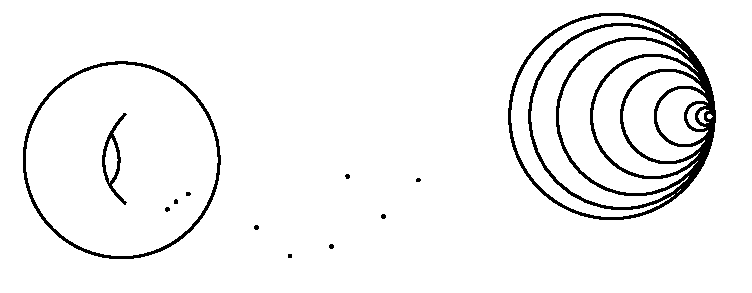
\includegraphics[width=0.5\textwidth]{critical_set.pdf}
\caption{Example of what the critical set might look like.}
\label{fig:critical_set}
\end{figure}
\end{exr}

\section{Properties of monopole Floer homology}

\subsection{$S^1$-equivariant homology}

Suppose we have a space with an $S^1$-action, like some finite CW-complex.

\begin{exm}
Consider $S^2$ with the $S^1$ action obtained by rotating around its axis. 
\end{exm}

\begin{exm}
$S^1$ acts on $S^3$ via the Hopf fibration.
This is a free action.
\end{exm}

In general the action might not be free, 
but up to homotopy equivalence we can always make it free with the Borel
construction. First we take the universal fibration
\begin{equation}
\begin{cd}
ES^1 \arrow{d}\\
BS^2
\end{cd}
\end{equation}
which means $ES^1$ is contractible, and the $S^1$ action on it is free. Then take
\begin{equation}
\begin{cd}
S_1\arrow[hook]{r}\arrow{d}&
S^3\arrow[hook]{r}\arrow{d}&
S^5\arrow[hook]{r}\arrow{d}&
\cdots\\
\pt\arrow[hook]{r}&
\CP^1\arrow[hook]{r}&
\CP^2 \arrow[hook]{r}&
\cdots
\end{cd}
\end{equation}
then in the limit we get $S^\infty$ mapping down to $\CP^\infty$, which is contractible
with free $S^1$-action.

Define the homotopy quotient by:
\begin{equation}
X//S^1 = X\times ES^1 / S^1
\end{equation}
Then the Borel $S^1$ equivariant cohomology is
\begin{equation}
H_{S^1}^*\left( X \right)\ceqq H^*\left( X//S^1 \right)
\end{equation}
This is functorial in the sense that if we have such an $S^1$ action on both $X$
and $Y$, then we have that $f:X\fromto Y$ gives us
\begin{equation}
f_*: H_{S^1}^*\left( Y \right) \fromto H_{S^1}^*\left( X \right)
\end{equation}
As a special case, if we have $X\fromto \pt$, we get a map
\begin{equation}
H_{S^1}^*\left( \pt \right) \fromto H_{S^1}^*\left( X \right)
\end{equation}
but we also have that
\begin{equation}
H_{S^1}^*\left( \pt \right) = H^*\left( BS^1 \right)
H^*\left( \CP^\infty \right) = \ZZ\left[ u \right]
\end{equation}
where $\deg u = 2$. 
All together, this means that there is a natural map 
$\ZZ\left[ u \right]\fromto H_{S^1}^*\left( X \right)$.
That is, $H_{S^1}^*\left( X \right)$ is a module over $\ZZ\left[ u \right]$.

\begin{thm}[Localization]
$u^{-1} H_{S^1}^*\left( X , \KK \right) \simeqq H^*\left( X^{S^1} ; \KK\right)
\tp_{\KK\left[ u \right]} \KK\left[ u^{-1} , u \right]$
for some field $\KK$, where $X^{S^1}$ is the fixed point set of the $S^1$ action 
on $X$.
\end{thm}

\begin{exr}
Compute the cohomology for the two examples above.
\end{exr}

\subsection{Formal properties of monopole Floer homology}

Consider some closed, oriented, connected manifold $Y^3$. 
Associate three objects to this. 
\begin{equation}
\begin{tikzcd}
\barr{\HM}_*\left( Y \right)
\arrow{r}{i_*}&
\checkk{\HM}_*\arrow{r}{\p_*}&
\hatt{\HM}_*\arrow[bend left]{ll}{p_*}
\end{tikzcd}
\end{equation}
The first is $\HM$ bar, the middle is $\HM$-to, 
and the third is $\HM$-from.\footnote{
These correspond to $\HF^\infty$, $\HF^+$, and $\HF^-$ respectively.}
These are modules over $\FF\left[ i \right]$, where $\deg u = -2$, 
and 
\begin{equation}
\checkk{HM}_*\left( Y \right) = 
\bdsum_{\fs \in \spin^x\left( Y \right)}
\checkk{\HM}\left( Y , \fs \right)
\end{equation}
We have the following dualities:
\begin{align}
\checkk{\HM}_*\left( Y \right) & \simeqq
\hatt{\HM}^*\left( -Y \right)
\\
\hatt{\HM}_*\left( Y \right) & \simeqq
\checkk{\HM}^*\left( -Y \right)
\\
\barr{\HM}_*\left( Y \right) & \simeqq
\barr{\HM}^*\left( -Y \right)
\end{align}
where $-Y$ is the manifold with opposite orientation.

As for gradings, each
$\checkk{\HM}_*\left( Y , \fs \right)$ is relatively graded over
$\ZZ / 2 d\left( \fs \right)\ZZ$ where $d\left( \fs \right)\in \NN$.

As a special case, let $Y$ be a homology sphere, so 
$H_*\left( Y \right)\simeqq H_*\left( S^3 \right)$, this means
there is only one potential $\spin^c$ structure, 
and $d$ of this structure is actually $0$. 
Then the relative grading in $\checkk{\HM}\left( S^3 \right)$ lifts to 
a canonical absolute $\ZZ$-grading.
So we can talk about the actual grading of an element 
whenever we consider a homology sphere. 

\begin{exm}
As a basic example we can just consider $Y = S^3$. 
\begin{align}
\barr{\HM}\left( S^3 \right) &= \FF\left[ u^{-1} , u \right]\\
\checkk{\HM}\left( S^3 \right) &= \FF\left[ u^{-1} , u\right] / \FF\left[ u \right]\\
\hatt{\HM}\left( Y \right) &= \FF\left[ u \right]
\end{align}
\end{exm}

\begin{exm}
If $Y$ is a homology sphere, then 
\begin{equation}
\barr{\HM}\left( Y \right) = \FF\left[ u^{-1} , u \right]
\end{equation}
up to grading shift. 
The group $\checkk{\HM}_*\left( Y , \fs \right)$ vanishes in degree low enough, 
and the map $i_*$ is an isomorphism in degree high enough.
\end{exm}

\begin{figure}
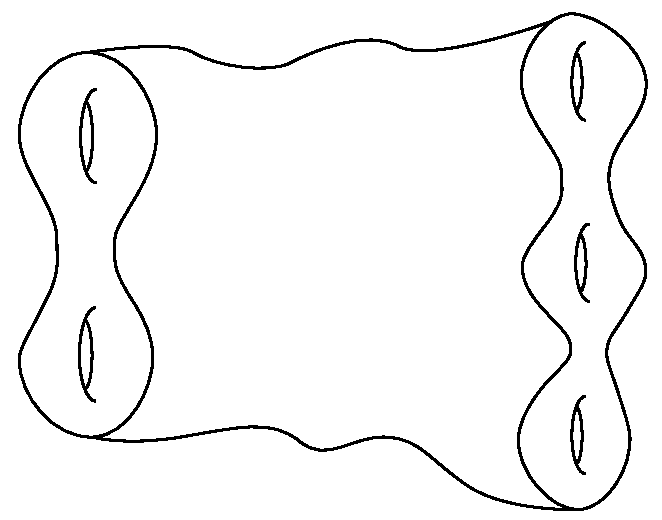
\includegraphics[width = 0.3\textwidth]{cobordism.pdf}
\caption{$W$ is bringing $Y_0$ to $Y_1$ in the sense that it has these
as its boundary.}
\label{fig:Y0_W_Y1}
\end{figure}

We now consider the functoriality of this construction.
If we have the situation in \cref{fig:Y0_W_Y1}, 
then this induces a map
\begin{equation}
\checkk{\HM}\left( W \right) : \checkk{\HM}_*\left( Y_0 \right) \fromto
\checkk{\HM}_*\left( Y_1 \right)
\end{equation}
This decomposes via the $\spin^c$ structures as
\begin{equation}
\checkk{\HM}\left( W \right) =
\bdsum_{s_W \in \spin^c\left( W \right)}
\checkk{\HM}\left( W , s_W \right)
\end{equation}

\begin{fact}
If we are again in the situation of 
\cref{fig:Y0_W_Y1}, then for
for $Y_0$ and $Y_1$ homology spheres, $b_1\left( W \right) = 0$, 
and $b_2^+\left( W \right)= 0$, 
then the map
\begin{equation}
\barr{\HM}\left( W , \fs_W \right): \barr{\HM}\left( Y_0 \right) 
\fromto \barr{\HM}\left( Y_1 \right)
\end{equation}
is an isomorphism of degree $\left( b_2\left( W \right) - c_1^2\left( \fs \right) \right) / 4$.
\end{fact}

\begin{proof}
This follows from $L^2$-hodge theorem.
\end{proof}

\begin{cor}
For $Y_0$ and $Y_1$ homology spheres, $b_2^+ = 0$ (negative definite)
we get the inequality:
\begin{equation}
h\left( Y_0 \right) \geq h\left( Y_1 \right) + \frac{1}{8} 
\left( 
\rk Q_W - \inf_{c}
\abs{Q_W\left( c , c \right)}
\right)
\end{equation}
where we are taking the infimum over characteristic classes $c$, that is, 
$c$ is $c_1$ of some $\spin^c$ structure.
\end{cor}

\begin{proof}
By doing surgery, we can assume $b_1\left( W \right) = 0$,
without changing $Q$. 
Then we have the following commutative diagram:
\begin{equation}
\begin{tikzcd}[column sep = large]
\barr{\HM}\left( Y_0 \right)
\arrow{d}{\cdot i_*}
\arrow{r}{\barr{\HM}\left( W , \fs_W \right)}&
\barr{\HM}\left( Y_1 \right)\arrow{d}{i_*} \\
\checkk{\HM}\left( Y_0 \right)\arrow{r}{\checkk{\HM}\left( W , \fs_W \right)}&
\checkk{\HM}\left( Y_1 \right)
\end{tikzcd}
\end{equation}
and this diagram commutes.
\end{proof}

\begin{thm}[Elkies]
$\rk Q_W \geq \inf_c \abs{Q_W\left( c , c \right)}$
where we range over characteristic $c$.
Furthermore, we have equality iff $Q_W = \left[ -1 \right]^n$.
\end{thm}

This is a theorem from number theory. This gives us the following:

\begin{cor}[Donaldson]
Suppose $X$ is closed, and $Q_x < 0$, then $Q_x = \left[ -1 \right]^n$.
\end{cor}

\begin{proof}
Remove two balls from $X$, and think of this as a cobordism from $S^3$ to itself.
Then since $h\left( S^3 \right) = 0$, by Elkies theorem, the intersection form is standard.
\end{proof}


\section{$S^1$-equivariant Morse (and Floer) homology}

We now actually define the monopole Floer homology.
Let $M$ be the configuration space 
\begin{equation}
\cC\left( Y , \fs \right) = 
\left\{ \left( B , \Psi \right) \right\} / \cG_0
\end{equation}
equipped with an additional $S^1$-action, where $S^1 = \cG / \cG_0$.
Then we have the Chern-Simons-Dirac functional
$f: M\fromto \RR / \left( 2\pi ^2 \ZZ \right)$.
The goal of this section is to compute some kind of
$S^1$-equivariant homology.

\subsection{Usual Morse homology}

Consider some smooth finite-dimensional manifold $X$, and take some Morse function
$f:X\fromto \RR$, then with some additional data, we can define a Morse
complex $C_*\left( X , f \right)$, which gives us the Morse homology
$H_*\left( X , \FF \right)$, which is the same as singular homology.

Now we want to provide a Morse-theoretic framework for $S^1$-equivariant homology.
The way we deal with this, is by using some-sort of blow-up construction. 
We can basically just think of this as polar-coordinates. 
Suppose $M$ is finite-dimensional and we have this $S^1$-action. 
Assume that the stabilizer of a point is either $\left\{ 0 \right\}$, or $S^1$.
The $\left\{ 0 \right\}$ case is irreducible, and an $S^1$-stabilizer is reducible.

\begin{exm}
Consider $\CC$ with multiplication by $S^1$. 
The origin is a fixed point, and everything else is free. 
Indeed, $\CC = \RR^{\geq 0}\times S^1 / \left\{ 0 \right\}\times S^1$, 
and then blowing up is just
\begin{equation}
\begin{cd}
\CC&
\CC^\sigma = \RR^{\geq 0}\times S^2
\arrow{l}{\pi}
\end{cd}
\end{equation}
to get a manifold with boundary.
Then in $\CC^\sigma$, the $S^1$-action is free, and $\CC^\sigma / S^1 = \RR^{\geq 0}$.
See \cref{fig:blowup_projection} to visualize this example.
\begin{figure}
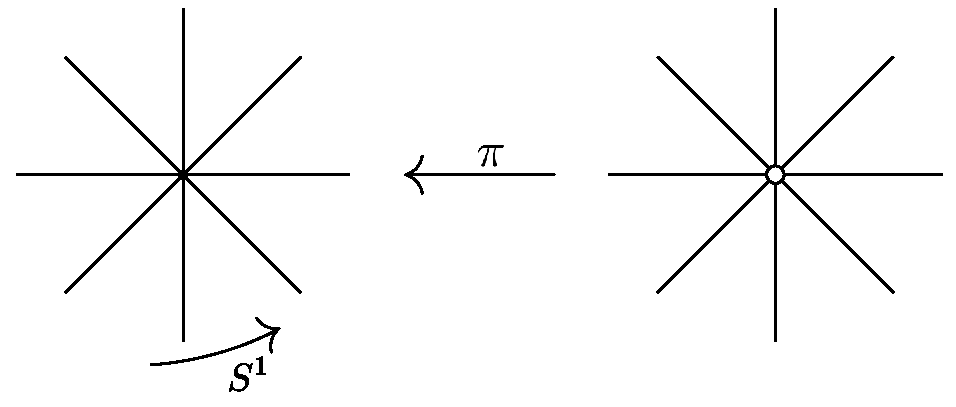
\includegraphics[width=0.5\textwidth]{blowup_projection.pdf}
\caption{The blow-up projects under $\pi$.}
\label{fig:blowup_projection}
\end{figure}
\end{exm}

\begin{exm}
Consider the space $\CC^n =\RR^{\geq 0} \times S^{2n-1} / \left\{ 0 \right\} \times S^{2n-1}$, 
then the blowup is
\begin{equation}
\left( \CC^n \right)^\sigma = \RR^{\geq 0} \times S^{2n-1} \fromto
\CC^n = \RR^{\geq 0} \times S^{2n-1} / \left\{ 0 \right\} \times S^{2n-1}
\end{equation}
and $\left( \CC^n \right)^\sigma / S^1 = \RR^{\geq 0} \times \CP^{n-1}$.
\end{exm}

\begin{exm}
In general, for $\left( M , g \right)$ with an $S^1$-action, 
we can suppose $S^1$ acts isometrically, 
then $M^{S^1}$ is the fixed point set of $S^1$ as in 
\cref{fig:fixed_points}.
\begin{figure}
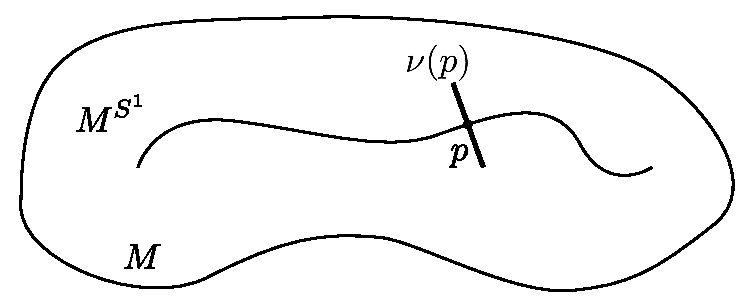
\includegraphics[width=0.4\textwidth]{fixed_points.pdf}
\caption{The fixed points $M^{S^1}$ and $\nu\left( p \right)$ for $p\in M$.}
\label{fig:fixed_points}
\end{figure}
then $S^1$ acts on $\nu\left( p \right)$, so
$\nu\left( p \right)$ has a natural almost complex
structure, now we blow-up fiber-wise, and then
\begin{equation}
\begin{cd}
M&
M^\sigma \arrow{l}{\pi}
\end{cd}
\end{equation}
where $S^1$ acts freely on $M^\sigma$.
$\pi$ is a diffeomorphism from 
$M^\sigma\minus \p M^\sigma \fromto M\minus M^{S^1}$.
\end{exm}

\begin{fact}
Consider $f:M\fromto \RR$ with an action of $S^1$. Then
$\restr{\grad f}{M\minus M^{S^1}}$ pulls back to a vector field $M^\sigma \minus \p M^\sigma$,
which extends naturally to a vector field on $M^\sigma$, 
$\left( \grad f \right)^\sigma$. 
Note that this is not the gradient of a function on $\sigma$.
\end{fact}

\begin{exm}
Consider $f:\CC^n\fromto \RR$ with an $S^1$-action, then
$f\left( z \right) = \lr{z , Lz}/2$ for $L$ some hermitian matrix.
In this case $\grad f\left( z \right) = Lz$, 
In polar coordinates $\left( r , \phi \right) \in \RR^{\geq 0} \times S^{2n-1}$.
Then for $r > 0$, 
\begin{equation}
\grad f\left( r , \phi \right) = 
\left( \Lam\left( \phi \right) r , L\phi - \Lam\left( \phi \right) \phi \right)
\end{equation}
where $\Lam\left( \phi \right) = \lr{\phi , L\phi}$.
This tells us that this formula defines an extension to $r =0$, 
the boundary of $M^\sigma$.
We can think of this heuristically in \cref{fig:fake_picture}.
\begin{figure}
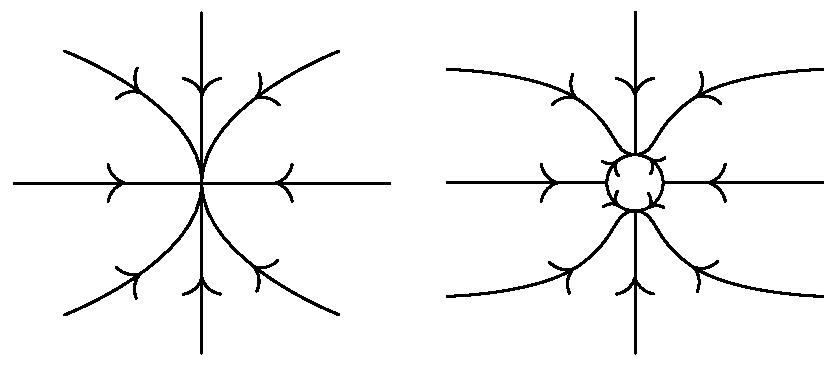
\includegraphics[width=0.5\textwidth]{fake_picture.pdf}
\caption{This is a ``fake picture'' of what is going on when
we extend $\grad f$.}
\label{fig:fake_picture}
\end{figure}
\end{exm}

\begin{rmk}
Critical points of $\left( \grad f \right)^\sigma$:
\begin{enumerate}
\item $\pi^{-1}\left( \text{ irreducible critical points of } \left( \grad f \right)\right)$
\item $\left( \text{reducible critical point, eigenvector of } L \right)$, 
\end{enumerate}
We know $L\phi = \Lam\left( \phi \right)\phi$, so
if you assume $L$ has simple spectrum $\lam_0 < \cdots < \lam_n$, each of them 
corresponds to a critical point in $\left( M^\sigma \right) / S^1$.
\end{rmk}

\subsection{Properties of $\left( \grad f \right)^\sigma$}

\begin{fact}
\begin{enumerate}
\item $\grad f^\sigma$ is tangent to $\p M^\sigma$ as in \cref{fig:gradient_flow}.
\begin{figure}
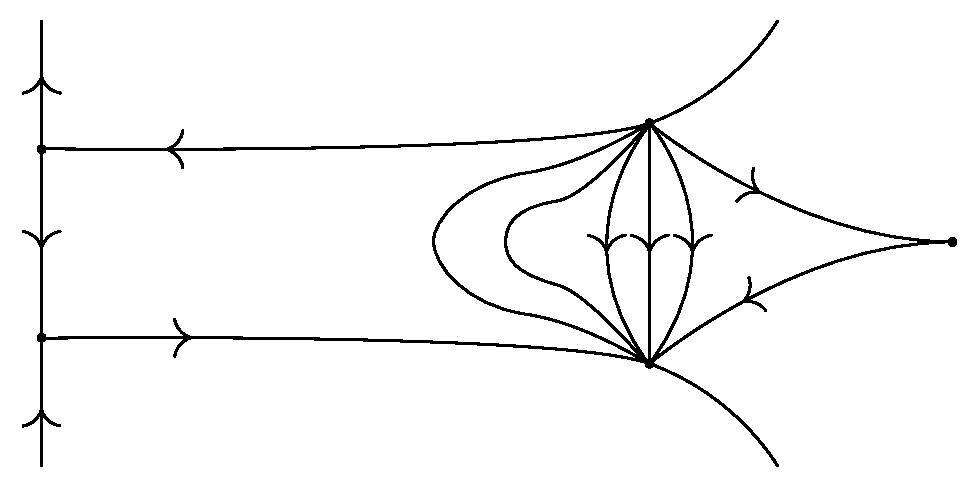
\includegraphics[width=0.5\textwidth]{gradient_flow.pdf}
\caption{The gradient flow $\grad f^\sigma$, and the corresponding critical points of
various indices. The upper point on the boundary is boundary-stable, and of index $1$. 
The bottom point on the boundary is boundary-unstable, and also of index $1$. 
Then the bottom critical point on the right is irreducible and of index $0$, 
and the top critical point is irreducible of index $2$. 
Then the middle critical point on the far right is of index $1$.}
\label{fig:gradient_flow}
\end{figure}
\item The flow is not Morse-Smale
\item A $1$-parameter family could break in $3$-components.
\end{enumerate}
\end{fact}

\subsection{Calculations}

Now we have a manifold with boundary, so we can calculate three different things:
homology of the boundary, homology of the space itself, and the homology of the space
relative to the boundary.

Take irreducible $C^0_k$, boundary-stable $C_k^s$, 
and boundary-unstable $C_k^u$.
The boundary maps are as follows.
We have
$\p^0_0: C^0_k\fromto C^0_{k-1}$,
which counts trajectories in $0$-dimensional moduli spaces.
Then we have $\p_s^0$, $\p_0^u$, $\p_s^u$,
and lastly we have
$\barr{\p}_s^s$, $\barr{\p}_u^s$, $\barr{\p}_s^u$, and $\barr{\p}_u^u$ which count on the boundary.
These are moduli spaces in $\p M^\sigma / S^1$.
In general, all of them drop the index by $1$, except for $\barr{\p}_u^s$, 
and $\barr{\p}_s^u$ which drops the index by $2$.

\begin{equation}
\checkk{C}_k = C_k^0 \dsum C_k^s
\end{equation}
then the boundary is defined by
\begin{equation}
\checkk{\p} =
\begin{pmatrix}
\p_0^0&\p^u_0 \barr{\p}_u^s \\
\p^0_s&\barr{\p}_s^s + \p_s^u \barr{\p}_u^s
\end{pmatrix}
\end{equation}

\begin{fact}
$\left( \checkk{X} , \checkk{\p} \right)$ is a chain complex whose homology computes
the homology of the underlying space $H_*\left( X \right)$. 
\end{fact}

To check this is a complex, we have to check $\left( \checkk{\p} \right)^2 = 0$, 
so we just have to write this out to get terms of the form
$\p^0_0 \p_0^0 + \p_0^u \barr{\p}_u^s \p_s^0$.
The idea is to look at ends of $1$-dimensional moduli spaces.

\begin{figure}
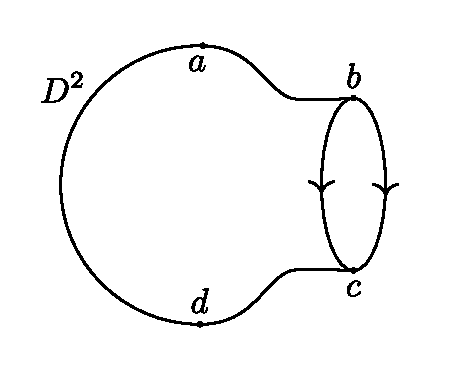
\includegraphics[width=0.4\textwidth]{critical_points.pdf}
\caption{The critical points $a$, $b$, $c$, and $d$ for the case $D^2$.}
\label{fig:critical_points}
\end{figure}

Let's compute $D^2$ as in \cref{fig:critical_points}.
In index $3$, we have $\FF\lr{a}$, for index $2$ we get $\FF\lr{b}$, and
in index $0$ we get $\FF\lr{d}$.
Then computing homology, we get $0$ in all degrees except $0$, where we get $\FF$.

Then
\begin{align}
\barr{C}_k = C^s \dsum C^u
&&
\hatt{C} = C^0 \dsum C^u
\end{align}
and then we define $\barr{\p}$ and $\hatt{\p}$ analogously.

\subsection{Definition of monopole Floer homology}

\begin{equation}
\begin{cd}
\cC\left( Y , \fs \right)&
\cC^\sigma\left( Y , \fs \right) = 
\left\{ \left( B , r , \Psi \right) \st 
r\in \RR^{\geq 0} , \norm{\Psi}_{L^2} = 1\right\}
\arrow{l}
\end{cd}
\end{equation}
Note that $\cG$ acts freely on $\cC^\sigma$.
Note that $\grad \cL$ extends to $\left( \grad \cL \right)^\sigma$.
Since the action is free, $\cC^\sigma\left( Y , \fs \right) / \cG$ 
is an infinite-dimensional manifold
with boundary, equipped with the vector field $\left( \grad \cL \right)^\sigma$. 
So now formally, we can just apply the construction of Morse-homology, to get
\begin{align}
\barr{\HM}\left( Y , \fs \right) &&
\checkk{\HM}\left( Y , \fs \right) &&
\hatt{\HM}\left( Y , \fs \right)
\end{align}
which are more or less obtained as before, by taking the homology of the boundary,
of the space, and of the space relative to the boundary.

\section{Pseudo-holomorphic curves}

\begin{defn}
Pseudo-holomorphic curves
\end{defn}

So if we have a pseudo-holomorphic curve 
$u:\Sigma \fromto \left( M , \om \right)$, then we can define the energy
\begin{equation}
E\left( u \right) - \int \abs{du}^2
\end{equation}

So $u$ is $J$-holomorphic iff $u$ minimizes $E\left( u \right)$
within its homotopy class.

For $\left( A , \Phi \right)$, we define
\begin{equation}
E\left( A , \Phi \right) = \frac{1}{4} \int \abs{F_{A^t}}^2 + 
\int \abs{\nab_A \Phi} +\frac{1}{2} \int
\left( \abs{\Phi}^2 + \frac{s}{2} \right)^2
\end{equation}
Then $\left( A , \Phi \right)$ solves the SW-equations iff it minimizes
$E\left( A , \Phi \right)$. 

\section{Triangulation conjecture}

Recall that we start with some configuration space
$\cC\left( T , \fs \right) = \left\{ \left( B , \Psi \right) \right\}$
with an action of the gauge group $\cG$, 
then we blow up the configuration space to get
\begin{equation}
\begin{tikzcd}
\cC\left( T , \fs \right) = \left\{ \left( B , \Psi \right) \right\}&
\cC^\sigma\left\{ \left( B , r , \psi \right) \st r\in \RR^{\geq 0} , \norm{\psi}_{L^2}= 1 \right\}
\arrow{l}{\pi}
\end{tikzcd}
\end{equation}
If we take the gradient of the Chern-Simons-Dirac functional:
\begin{equation}
\grad \cL\left( B , \Psi \right) = 
\left( \frac{1}{2} * F_{B^t} + \rho^{-1}\left( \Psi \Psi_0^* \right) , 
D_B \Psi\right)
\end{equation}
we can explicitly extend this as:
\begin{equation}
\left( \grad \cL \right)^\sigma \left( B , r , \psi \right) = 
\left( \frac{1}{2} * F_{B^t} + r^2 \rho^{-1}\left( \psi \psi_0^* \right) , 
\Lam\left( B , \psi  \right)r , D_B\psi - \Lam\left( B ,\psi \right) \psi\right)
\end{equation}

We have the following types of critical points of $\left( \grad \cL \right)^\sigma$:
\begin{enumerate}
\item Irreducible critical points of 
$\grad \cL$
\item Reducibles $\left( B , 0 , \psi \right)$
with $\left( B , 0 \right)$ a criticalm points of $\grad \cL$
and $\psi$ is a unit eigenvector of
$D_B / S^1$.
\end{enumerate}

Generically $D_B$ has a simple spectrum,
so we have eigenvalues
$\cdots < \lam_{-1} < 0 < \lam_0 < \lam_1< \lam_2 < \cdots$
where $\lam_i$ corresponds to one critical points $c_i$. 
Then we have the following facts:
\begin{fact}
\begin{enumerate}
\item $c_i$ is stable iff $\lam_i > 0$
\item Two consecutive critical points $\lam_i$ and 
$\lam_{i+1}$ differ in grading by $2$.
\end{enumerate}
\end{fact}

\begin{exm}
Consider $\checkk{C}\left( S^3 \right)$. 
We know that positive scalar curvature implies there are no irreducible solutions, 
and since $b_1\left( Y \right) = 0$, we have exactly one reducible solution.
Since grading differs by $2$, there's no room for a differential here.
\end{exm}

\begin{exm}
Consider $\checkk{C}$ of the Poincar\'e homology 
sphere. Again we have positive scalar curvature, so there are no irreducible solutions, 
and $H_1\left( Y \right)= 0$. 
So this is basically the same as the previous example.
\end{exm}

\begin{exm}
We can also calculate $\checkk{C}\left( \Sigma\left( 2,3,7 \right) \right)$. 
There is just one reducible solution, only now there are also two irreducible solutions, 
and each comes with a trajectory $\FF\dsum \FF\fromto \FF$, 
so we have a nontrivial differential. 
\end{exm}

\begin{thm}[Manolescu]
The triangulation conjecture is false 
in higher dimensions, that is, for $n\geq 5$, there exists
a topological manifold $M^n$ not homeomorphic to a simplicial 
complex.
\end{thm}

As it turns out, this is equivalent to a problem in low dimensional topology.
Consider the homology cobordism group
\begin{equation}
\Theta_H^3 =
\left\{ Y \text{oriented, }\ZZ HS^3 \right\} / \sim
\end{equation}
where two $Y_0\sim Y_1$ both
$\ZZ HS^3$ iff $y_i \inj W$ as in 
\cref{fig:Y0_W_Y1}.
This is an equivalence in $H_*\left( \cdot , \ZZ \right)$.

\begin{rmk}
$\Theta_H^n = 0$ for $n\neq 3$ (in the PL category).
\end{rmk}

As it turns out, $\Theta_H^3 \neq 0$. 
There is a homomorphism 
\begin{equation}
\mu: \Theta_H^3\fromto \ZZ / 2\ZZ
\end{equation}

\begin{thm}[Rokhlin]
Suppose $X^4$ is a smooth spin,
then $16$ divides the signature $\sigma\left( X \right)$.
\label{thm:rokh}
\end{thm}

\begin{rmk}
For $X$ spin, $Q_X$ is even, so for algebraic reasons
we know that $8$ divides $\sigma\left( X \right)$. 
The cool thing is then that since we insist the space is smooth, we
can boost this to be a $16$.
\end{rmk}

Suppose we have that $Y$ is a $\ZZ H S^3$. 
Then it is a classical result that any such $Y$ bounds
some $W$ which is also spin. 
Then define
\begin{equation}
\mu\left( Y \right) = \frac{\sigma\left( W \right)}{8}\in \ZZ / 2\ZZ
\end{equation}
This is well defined, since if we have some other $W'$, 
we can glue them together along $Y$, 
and we get a closed spin manifold, so $16$ divides the signature
$\Sigma\left( W\minus W' \right) = \sigma\left( W \right) - \sigma\left( W' \right)$, 
so its divisibility is indeed well defined.

\begin{exm}
$S^3$ is the boundary of $B^4$, so $\mu\left( S^3 \right)= 0$. 
For the Poincar\'e homology sphere, we get that this is the boundary of $P_{E_p}$.
Then $T^*S^2$ gives us the $E_8$ Dynkin diagram, so we get $\mu$ of Poincar\'e
to be $1$.
\end{exm}

\begin{thm}[Galeski-Stern-Matumoto]
The triangulation conjecture is false iff
$\mu$ does not split, that is, 
there are no elements $\left[ Y \right]\in \Theta_H^3$ with order $2$, 
and $\mu = 1$.
\end{thm}

So this is the fact that Manolescu showed:

\begin{thm}[Manolescu]
There exists a $\b:\Theta_H^3\fromto \ZZ$, which is not a homomorphism, such that
\begin{enumerate}
\item $\b\left( \left[- Y \right] \right) = -\b\left( \left[ Y \right] \right)$
\item $\b\left( \left[ Y \right] \right) = \mu\left( \left[ Y \right] \right)\pmod{2}$
\end{enumerate}
\label{thm:mano}
\end{thm}

This implies the triangulation conjecture is false because of the following. 
Suppose the homomorphism splits. 
Then we have an element $Y$ or order $2$, so
$2\left[ Y \right] = 0$, 
which is the same as $\left[ Y \right] = -\left[ Y \right]$.
Then we get $\b\left( \left[ Y \right] \right) = \b\left( -\left[ Y \right] \right)$,
but this is an integer, so we must have that $\b\left( Y \right) = 0$, 
which means $\mu\left( Y \right) = 0$.

Recall in monopole Floer homoloy 
we get this invariant $h\left( Y \right)\in \ZZ$
called the Froyshov invariant.
This gives us a map 
$h:\Theta_H^3 \fromto \ZZ$,
but this doesn't have the second property from \cref{thm:mano}.
To see this, we can simply check the example
$\Sigma\left( 2 , 3 , 7 \right)$ from before.

So we need to exploit an extra symmetry of the Seiberg-Witten equations
in the presence of spin structures.
This extra symmetry is:
\begin{equation}
\Pin\left( 2 \right)= S^1 \un \cJ S^1 \subeq \HH
\end{equation}
This is like a Hopf link as in \cref{fig:pin_link}
\begin{figure}
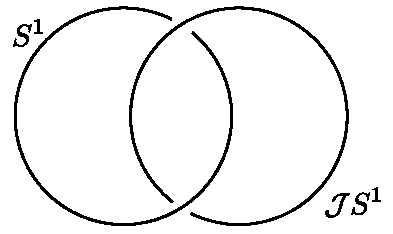
\includegraphics[width=0.4\textwidth]{pin_link.pdf}
\caption{Hopf link of $S^1$ and $\cJ S^1$.}
\label{fig:pin_link}
\end{figure}

Returning to \cref{thm:rokh},
we have a $\spin^c$ structure
$S = S^+ \sum S^-\fromto X^4$, where both $S^{\pm}$
have complex rank $2$.
Then the Dirac operator
$D_A^+:\Gamma\left( S^+  \right)\fromto \Gamma\left( S^- \right)$
has index
\begin{equation}
\ind D_{A^t}  = \dim \ker - \dim \coker = 
\frac{1}{8}\left( c_1^2\left( S^+ \right) - \sigma\left( X \right) \right)
\end{equation}
We have an action of $\cJ$ on $S^{\pm}$ where
$\cJ^2 = -\id_{S^{\pm}}$, and $\cJ$ is complex antilinear. 
Then this implies $S^{\pm}$ are $\rank_{\HH} = 1$
quaternionic vector bundles.

There is a distinguished connection
$A_0$, the spin connection so that
\begin{equation}
D_{A_0}^+ \left( \Psi \cJ \right) = 
\left( D_A \Psi \right) \cJ
\end{equation}
is quaternionic linear. This is because 
\begin{equation}
\Spin\left( 3 \right) = \SU\left( 2 \right)
\left\{ 
\begin{pmatrix}
a & - \barr{b} \\ b & \barr{a} \st 
\abs{a}^2 +\abs{b}^2 = 1
\end{pmatrix}
\right\}
\end{equation}
acts on $\CC^2 = \HH$, where we have identified
$\left( z,w \right)$ with $z + \cJ w$.
Then we have that $\SU\left( 2 \right)$ and $\cJ$ both act on $\HH$ and commute.

This means
$\ker A_{A_0}^+$ is a quaternionic vector space
(if $X$ is spin), and similarly for the cokernel where
$\coker A_{A_0}^+ = \ker D_A^-$.

Then in $2\ZZ$, we get
\begin{equation}
\ind D_{A^t} = \frac{1}{8}\left( c_1\left( S^+ \right)^2 - \sigma\left( X \right) \right)
= -\frac{1}{8}\sigma\left( X \right)
\end{equation}
and $S^+$ is congruent to its conjugate, which means $16$ divides $\sigma\left( X \right)$
as desired.

In the case of a three manifold, $Y$
with a spin structure, $S\fromto Y$,
we have an action of $\cJ$ on $S$, and
we get $\cJ^2 =-\id_S$, and $\cJ$ is complex antilinear.
For $B_0$ the spin connection, we get that $D_{B_0}:\Gamma\left( S \right)\fromto \Gamma\left( S \right)$
is quaternionic linear.

Now for $\left( B, \Psi \right)\in \cC\left( Y , \fs \right)$, 
we have
\begin{equation}
\cJ\left( B , \Psi \right) = \left( \barr{B }, \Psi \cJ \right)
\end{equation}
where $B = B_0 + b$, and $\barr{B} = B_0 - b$. 
Then we have
\begin{equation}
\cJ^2 \left( B , \Psi \right) = \left( B , -\Psi \right) \sim \left( B , \Psi \right)
\end{equation}
are gauge equivalent. 
This means the function $\cL$ is invariant under the $\Pin\left( 2 \right)$ action
on $\cC\left( Y , \fs \right)$ since we have this extra $\cJ$.

So now we might try to do some sort of $\Pin\left( 2 \right)$ equivariant Floer homology.
We can formally define this to be a module over
\begin{equation}
M_{\Pin\left( 2 \right)}\left( \pt \right) = 
\FF\left[ V , Q \right] / Q^3 = H^*\left( B\Pin\left( 2 \right) \right)
\end{equation}
where $\deg V = -4$, and $\deg Q = -1$. 
Note that this contains $\FF\left[ Q \right] / Q^3$, which is $H_*\left( \RP^2 \right)$, 
so this is where $\RP^2$ comes into this picture. 

In the $\spin^c$ case, $D_B$
has simple spectrum, so $\lam_i$ corresponds to critical points,
which is the unit sphere eigenspace modulo $S^1$. 
In our case, $D_{B_0}$ has simple (in the quaternionic sense) spectrum,
so an eigenvalue $\lam_i$ corresponds to
$S^3 / S^1 = S^2$ where $\cJ$ acts on this, so we get $\RP^2$.

% >>><<<
\bibliography{math}
\end{document}
